\documentclass[11pt,a4paper]{article}
\usepackage[T1]{fontenc} 
\usepackage[utf8]{inputenc}
\usepackage{fourier}
\usepackage[english]{babel} 
\usepackage{amsmath,amsfonts,amsthm} 
\usepackage{threeparttable}
%\usepackage{rotating}

%hyperlinks
\usepackage{hyperref}
\usepackage{url}

\usepackage{color,enumitem,listings,units,subcaption,caption,float,natbib}
\usepackage{booktabs}
\usepackage{tabularx}
\usepackage{multirow}


\usepackage{graphicx, lscape}
\usepackage[left=2.54cm, right=2.54cm, top=3cm, bottom=2.8cm]{geometry}


\begin{document}
	
\title{{\Huge Macroeconomic Effects of Oil Price Shocks: \\
		\vspace{0.5em}
		 a FAVAR Approach.}
	\vspace{3em}}

\author{{\LARGE Marco Goretti
	\footnote{Faculty of Business and Economics, University of Lausanne, Lausanne, Switzerland, marco.goretti@unil.ch}}
	\\ {\large University of Lausanne  }
	\and {\LARGE Frédéric Martenet
	\footnote{Faculty of Business and Economics, University of Lausanne, Lausanne, Switzerland, frederic.martenet@unil.ch}} 
	\\ {\large University of Lausanne  }
	\and {\LARGE Simon Tièche
	\footnote{Faculty of Business and Economics, University of Lausanne, Lausanne, Switzerland, simon.tieche@unil.ch}}
	\\ {\large University of Lausanne  }
}
	
\date{\vspace{3em}{\Large \today}}

\maketitle

\thispagestyle{empty}

\vspace{3em}
\begin{abstract}
	{\noindent\large 
		We study the macroeconomic consequences of an exogenous oil price shock. We first estimate a state of the art Structural VAR model. We then take advantage of a large amount of data and estimate a Factor-Augmented VAR model.
		Both model indicate that such a shock has a moderate and brief impact on economic activity.
		However, using the FAVAR yields effects that are greater and more persistent than using the SVAR. This indicates that augmenting the SVAR to a FAVAR, and, therefore, taking advantage of the information contained in a huge data set describing the economy allowed us to estimate structural impulse response functions that are closer to the true ones. 
		
		{\large \vspace{3em} \noindent\textbf{Keywords:} Business Cycles, FAVAR, Oil shocks,   SVAR}

	}
\end{abstract}




\vspace{3.5cm}
\begin{center}
\url{https://github.com/mgoretti/macroeconometrics-favar}
\end{center}

\clearpage
	
	\setcounter{page}{1}

\section{Introduction} % The \section*{} command stops section numbering

Oil is the major source of primary energy in the world. It plays a key role in trade  via its use by vehicles and planes to transport goods and people.  
It is also an important factor of production for firms from very diverse sectors. 
A key aspect of oil  is the volatility of its price: it can vary a lot in a short period of time in response to unexpected events. The usual worldwide reference price is the crude oil Brent. The Brent nominal price was more or less stable around \$20 per barrel during the 1990s. It then began a steady increase to reach a peak of \$145/barrel in July 2008. During the financial crisis and its aftermath, it dropped below \$40 a barrel and somewhat stabilized above \$100 between February 2011 and the Summer 2014. Since then,  a strong downward trend drove the price down, even below \$30 a barrel. The recent decrease is usually explained by a voluntary high production  from the OPEC countries and the development of new technologies such as fracking. 


Economists have been interested in the effects of oil price  since the two oil crises of 1973 and 1979. An unexpected sharp increae in oil price is a negative shock for the economy. Firms are hurt as their production costs unexpectedly increase in a short period of time. 
Conventional wisdom indicates that such a shock should have a negative impact on economic activity. 
The literature on oil and its impact on the economy has demonstrated that oil price and economic growth are indeed linked \citep{hamilton1983oil, hamilton2003oil, hamilton2011historical}.

A common framework to analyze the consequences of unexpected shocks on the economy are the Structural Vector-Autoregressions (SVARs) (due to \citealp{sims1980macroeconomics}): a methodology that allows the macroeconomist to identify the impacts of exogenous shocks. 
This class of models considers a small number of variables describing an economy and estimates how they behave and interact. 
Under some assumptions, it allows the macroeconomist to shock one variable and analyse the impacts of this shock on the other variables.
These models have been widely used in many different context (for oil price shocks, see \citealp[chp. 7]{gali2010international}, for monetary policy, see \citealp{christiano1999monetary}).

More recently, a similar framework called Factor-Augmented Vector-Autoregressions (FAVAR)  has been developed \citep{bernanke2005factor}. 
It allows to take advantage of a large amount of information, which is not possible with VARs as they usually include very few variables. This methodology has also been used to identify the effects of oil price shocks \citep{aastveit2014oil, aastveit2015drives}.   

Our aim is to estimate the macroeconomic effects of an exogenous oil price shock. In a first step, we use a low-dimensional state of the art SVAR. 
In a second step, we take the advantage of a large data set and augment our VAR with so-called factors. 
We then compare the results of the SVAR and the FAVAR.

Our results indicate that an unexpected oil price shock has a brief negative impact on output growth,  four quarters after the shock. Total employment is also negatively affected four quarters after the shock. The magnitude of these impacts is low, this indicates that oil price plays a relatively minor role in business cycles, which is consistent with the existing literature.
However, results from both models are contrasting. While the SVAR indicates that none of these effects is statistically significant at the 90\% level, the FAVAR estimates effects that are significant, greater and more persistent than the ones of the SVAR. This indicates that augmenting the SVAR to a FAVAR, and, therefore, taking advantage of the information contained in a huge data set describing the economy, allowed us to estimate structural impulse response functions that are closer to the true ones. 

Section \ref{sec:method} presents our methodology, section \ref{sec:data} describes the data we use, section \ref{sec:results} describes our results and section \ref{sec:conclusion} concludes. Tables, graphs and supplementary materials are available in the appendix. 
%The entire robustness checks are available on our repository. 





%------------------------------------------------
\section{Methods}
\label{sec:method}
%------------------------------------------------

\subsection{Structural Vector Autoregression (SVAR)}

% intro : 

In a first step, we estimate the macroeconomic impacts of an exogenous oil price shock in a SVAR framework. We consider the oil price, $O_t$, and a vector $X_t$ that includes real GDP, employment, inflation and the interest rate. The VAR($p$) representation is 

{\footnotesize
\begin{align*}
 \begin{pmatrix} O_t \\ X_t \end{pmatrix} = 
A_1 \begin{pmatrix} O_{t-1} \\ X_{t-1} \end{pmatrix} +
A_2 \begin{pmatrix} O_{t-2} \\ X_{t-2} \end{pmatrix} +
\ldots +
A_p \begin{pmatrix} O_{t-p} \\ X_{t-p} \end{pmatrix}
+ \eta_t 
\qquad \text{or} \qquad
A(L) \begin{pmatrix} O_t \\ X_t \end{pmatrix} = \eta_t
\end{align*}
}

with $A(L) = 1 - A_1 L - A_2 L^2 -  \ldots - A_p L^p$, $L$ is the lag operator and $\eta_t$ is a disturbance with mean zero and covariance $\Sigma_\eta$. 
Note that the VAR considers the innovations $\eta_t$, but that for the purpose of our analysis we are interested in the \emph{structural} shocks $\epsilon_t$. The SVAR methodology assumes that the innovations are a linear combination of the unobserved structural shocks, $i.e.$ that the space of the innovations $\eta_t$ spans the space of the structural shocks $\epsilon_t$ :  

{\footnotesize \begin{equation}
\eta_t = H\epsilon_t, \label{eq:ino}
\end{equation}}

\noindent
where the structural shocks are uncorrelated.
Substituting this new assumption in the VAR representation and rearranging yields the structural moving average representation 

{\footnotesize $$ \begin{pmatrix} O_t \\ X_t \end{pmatrix}
= D(L) \epsilon_t,$$}

\noindent
where  $D(L) \equiv A(L)^{-1}  H$. 
The above expression represents the dynamic impact of the structural shocks on the present and future values of our five variables of interest.
The structural impulse response functions (IRFs) is the time path of the impact of a unit increase in the structural shocks on the five variables. Let $D_h$ denote the $h^{th}$ lag matrix coefficients in $D(L)$. Then $D_{h,ij}$ is the impact on the $i^{th}$ variable of a unit increase of the $j^{th}$ structural shock after $h$ periods. Thus, the structural IRF of the $i^{th}$ variable in response to the $j^{th}$ structural shock is the sequence 

{\footnotesize \begin{align*}
SIRF_{ij} = \{ D_{h,ij} \}, \qquad h = 0,1,2,3,\dots 
\end{align*}}

However, we still need to determine the relation between the innovations and the structural shocks, $i.e.$ assume a form for $H$.
This is known as the SVAR identification problem. From equation \eqref{eq:ino}, we have
$ \Sigma_\eta  = H \Sigma_\epsilon H', $
where $H$ contains $n^2$ free parameters and $\Sigma_\epsilon$ contains $n$ free parameters. As a covariance matrix is symetric, it is reduced to $n(n+1)/2$. We can get rid of $n$ free parameters by normalizing the scale of shocks, $i.e.$  $\Sigma_\epsilon = I$. This leaves $n(n-1)/2$ restrictions to impose in order to identify $H$.
To do so one can use short-run restrictions as proposed by \cite{sims1980macroeconomics}, long-run restrictions or sign restrictions. 
{\color{black}The most natural way in our case is to impose short-run restrictions.}

% identification : 
To identify the effect of an unexpected structural oil shock (through the impulse response function (IRF), we impose short-run restrictions. This is equivalent to ordering the variables in such a way that the first innovation responds within a period only to the first structural shock , the second innovation responds only to the first and second structural shocks, and so forth. $H$ is then a lower triangular matrix than can be computed as $H = Chol(\Sigma_\eta)\Sigma_\epsilon^{-\frac{1}{2}}$, where $Chol(\cdot)$ is the Cholesky factorization.



%To identify the effect of an unexpected structural oil shock on real and nominal data (through the impulse response function (IRF)), one may use a SVAR for multiples reasons. 
%First, the structural shock space to a vector of time series $Y_t$ spans the space of the structural shock.{\color{black} Hence, the task of identifying the structural shock \textbf{of interest} reduces to the task of finding the linear combination of the structural shock. }



%To do so one can use short-run restrictions as proposed by \cite{sims1980macroeconomics} or long-run restrictions. 
%{\color{blue}The most natural way to proceed in our case is to impose short-run restrictions.} This is equivalent to ordering the variables in such a way that the first innovation responds within a period  only to the first structural shock , the second innovation responds only to the first and second structural shocks, etc. $H$ is then a lower triangular matrix than can be computed as $H = Chol(\Sigma_\eta)\Sigma_\epsilon^{-\frac{1}{2}}$, where $Chol(\cdot)$ is the Cholesky factorization.


Doing this implies that we treat the structural oil price shock as exogenous, $i.e.$  the oil price $O_t$ responds within a period only to oil price shocks $\epsilon_{t}^{oil}$ and nothing else, $\eta_{1,t} = \epsilon_{t}^{oil}$.
The literature considers that this holds as any unexpected change in oil prices is, in general, exogenous to developments in the U.S. economy. %  \cite{stock2015factor}. 
The main motivation is that if unexpected changes in oil arise from unexpected developments in supply then those changes are specific to oil supply, and thus can be thought of as oil supply shocks. 
So an unexpected increase in the  price of oil can be interpreted as an exogenous oil price shock. 
%Then, we can identify IFR by looking at the cycles of of the oil price (log). 
As we only are interested in the effect of the oil shock on the economy,  we can simply order oil price first in the Cholesky decomposition. Thus, equation \eqref{eq:ino} becomes 


{\footnotesize \begin{equation}
\eta_t = 
\begin{pmatrix} 1 & 0 \\ H_a & H_b \end{pmatrix}
\begin{pmatrix}  \epsilon_t^{oil} \\ \tilde{\eta}_t \end{pmatrix}, \label{eq:ino2}
\end{equation}}
The order of the remaining variables does not matter for the purpose of identifying and estimating the structural IRFs with respect to the oil shock.
 
In a general way, structural VARs are widely used to trace out the effect of shocks on the economy. Oil price shocks have been analyzed using the above framework \cite[chp. 7]{stock2015factor,gali2010international}.
However, the information sets usually used in these empirical models lead to a potential major problem: 
measurement innovations are likely to be contaminated if the reality has some information that is not in the VAR. 
For example, central banks base their monetary policy decisions on a much wider range of information rather than a few macroeconomic variables. 
As a consequence, we need to construct a model that combines the standard structural VAR analysis with recent developments in factor analysis for large data sets.
% Factor-Augmented VAR models are discussed in the next subsection.



%{\color{red} If place and time allows : 
%
%Other identification with supply demand
% \cite{kilian2009not} 
% 
% But we don't give a fuck as we don't do it}

\subsection{Factor-Augmented Vector Autoregression (FAVAR) \label{subsec:favar}}

The FAVAR model adds artificial variables, called factors, summarizing a dataset of additional information to the previous SVAR model. 
If we look at $m$ observed variables describing for example the US economy, with $m$ very large, we can summarize most of the  information of this huge database in $k$ unobservable variables called factors, with $k$ very small. These factors may be seen as indices of economic activity or credit conditions. 
To compute those factors, two approaches dominate the literature. The first one is by using common components through the Principal Component Analysis (PCA). 
Another way of calculating the factors is by using a Bayesian likelihood approach. Actually, none of those methods dominates the other. In this paper, we use principal component analysis to calculate factors as suggested by \cite{stock2015factor}. 
We then \emph{augment} our initial VAR with the estimated factors. 
The VAR($p$) representation of our model is now  


{ \footnotesize \begin{align*}
 \begin{pmatrix} O_t \\ X_t \\ F_t \end{pmatrix} = 
A_1 \begin{pmatrix} O_{t-1} \\ X_{t-1} \\ F_{t-1} \end{pmatrix} +
A_2 \begin{pmatrix} O_{t-2} \\ X_{t-2}\\ F_{t-2} \end{pmatrix} +
\dots +
A_p \begin{pmatrix} O_{t-p} \\ X_{t-p}\\ F_{t-p} \end{pmatrix}
+ \eta_t 
\qquad \text{or} \qquad
A(L) \begin{pmatrix} O_t \\ X_t \\ F_t \end{pmatrix} = \eta_t,
\end{align*} }

\noindent
where $F_t$ is a vector that contains the factors estimated with principal component analysis. 
This methodology has also been used to identify the effects of oil price shocks \citep{aastveit2014oil, aastveit2015drives}. 

%\paragraph{Principal Component Analysis} The first step to calculate factors using PCA is to center and standardize the database - i.e.  removing the influence of location and scale from variables in the raw data. The second step consists of calculated the variance-covariance matrix of the centered and standardized data. Then we calculate the eigenvector of this variance-covariance matrix and keep the $k^*$ largest eigenvalues. Hence we get a $k^* \times 1$ vector of eigenvalues ranked by the largest to the lowest value. The eigenvector with the highest eigenvalue is the principle component of the data. The next step consists of project the data using the vector $k^*$to obtain a new database ($W$) from the selected $k^*$ eigenvalues. Finally, we transform the original database via $W$ to obtain a $k^*$-dimensional feature subspace of $Y$, the vector of variables of interest. Hence, we can summarize most of the unobserved information containing in our raw database by assuming observable unobservable factors. Doing so permits us to deal with contamination in  measurement of the innovations as we account for information that a VAR or SVAR cannot have and permits us to get IRF that can be observed only for the included variables, which generally constitute only a small subset of the variables. Results are discussed in section \ref{sec:results}.
\vspace{1em}
\noindent\textbf{Principal Component Analysis} Our PCA algorithm works on data that was previously centered and standardized, which removed the influence of location and scale. \newline
The method calculates the eigendecomposition of the variance-covariance matrix of the dataset, then sorts the eigenvalues by magnitude (as it is proportional to the variance explained by the eigenvector). We then keep the top $k$ eigenvectors of the highest eigenvalues and generate the factors by projecting the dataset on them, which yields $k$ new variables (the factors) as a linear combination of the previous variables in the dataset. \newline
It is important to notice that the generated factors are uncorrelated (orthogonal) and they explain the most variance (thus information) of the original dataset with the least possible number of variables, by construction. This reduces overfit by drastically reducing the number of variables in the model while allowing us to include more information. 




%------------------------------------------------
\section{Data}
\label{sec:data}
%------------------------------------------------

The five variables used in the SVAR are a producer price index of oil,  real GDP, total nonfarm employment, a consumer price index and the Effective Federal Funds Rate. Descriptive evidence of these variables is provided in figure \ref{fig:descriptive}. 
The series were transformed to be  integrated of order zero. \footnote{These transformation are similar to \cite{stock2015factor}, they justify those with unit root tests and judgment.  We provide the results of Augmented Dickey-Fuller tests  in Table \ref{tab:DF} that confirms the stationarity of the series.  Moreover, following \cite{stock2015factor}, we remove the low-frequency trends using a Bi-Weight filter.   }
The series were subsequently standardized to have unit variance and mean zero.

We compute the factors using the data set provided by \cite{stock2015factor}. It contains 207 time series  mainly describing the US economy.
After removing the series that are aggregates of others and dropping the ones with missing values, we are left with a final data set of 106 variables. More details on data and their transformations are available in the appendix.

%------------------------------------------------
\section{Results and Discussion}
\label{sec:results}
%------------------------------------------------


\textbf{Parameter tuning }  Cross-validation was used to tune the number of lags in both models and also for the number of factors in the FAVAR model. The method is particularly useful to avoid overfit. It generate splits of the dataset in a training and a testing set (we used proportions $\frac{4}{5} \, \frac{1}{5}$ in our setting) and then, for each split, forecasts the test set using only the training set and finally averages the result of the loss function (we used root mean squared error) over all the splits (5 test sets) and the simulations (100 different combinations of splits). In the case of time series, the standard method becomes a bit different since removing the observations in the test set would severely reduce the training data (as most of the lag information would not be available anymore). We used the methodology of \cite{bergmeir} by generating all the regressions and then removing the regressions that contained the test set as the dependent variable. This allowed us to not lose most of our training set by keeping the information in the test set as lags. It can be seen in figure \ref{fig:CV}.A that after 2 lags, the train error keeps going down ($R^2$ increases) while the test error goes up (sign of overfit). \\
This allowed us to opt for 2 lags in our model. Nevertheless, we performed other lags test as robustness check, as it can be seen in Table \ref{tab:IC}. We can see that our parameter is close to what the BIC and HQIC suggest. The same procedures allows to find that the best number of factors for the FAVAR is 2 which is consistent with the criterion suggested by \cite{onatski2010determining}. Figure \ref{fig:CV}.B shows the explained variance as a function of the number of factors

\subsection{SVAR}

Figure \ref{fig:SVAR_irf} presents the structural IRFs for the selected variables (oil price growth, real GDP growth, total employment growth and change in inflation) with respect to a temporary oil shock at time $t =1$. Because of the unit standard deviation normalisation, a unit oil price shock increases the growth of oil prices by one standard deviation. Then, oil price growth increases concavely (less and less) until quarter 4 from where the growth of oil price reverts until it stabilizes (quarter 8), $i.e.$ if the mean growth rate is 10\% and its standard deviation 5\%, the oil price growth jumps to 15\% in quarter 1, decreases until 9\%  at quarter 4 and then increases again until stabilizing back at its mean in quarter 8.
% The oil shock lasts 4 quarters on the oil price. 
The inflation pattern is really close to the oil price one, which confirms that the oil price is a strong determinant of the inflation for a country like The United States. When the shock arises, change in inflation (relative to its mean level) suddenly becomes positive for a period, then becomes negative until quarter 4 and finally reverts back to the mean. Overall, we can say that change in inflation follows oil price growth quite well, as expected.

The shock does not have a significant effect on Real GDP growth in quarter 1. Then, the effect decreases until becoming almost significative in quarter 4. After that it grows again and stabilises at its mean. 
We do not observe a significant effects on growth of employment. 


%
%our Structural VAR suggests that an oil shock has (1) a one-for-one impact on the oil price in the very short-run (as constructed in the model) and that the shock is absorbed after 4-5 periods ($\approx$ one year and a half), has (2) a small positive impact on the real gdp in the short-run and a negative impact after 4-5 quarters, has (3) a quiet one-for-one impact on the inflation in the very short-run and an impact that becomes negative after 3-4 quarters and has (4) a positive effect on the employment in the short-run and a negative impact on the employment in the medium-run. The shock is absorbed after 9-10 quarters. Those results suggest that the oil price is a strong determinant of the inflation but that its effect on the economy differs. 
%If the demand for oil increases, it is likely the case that the demand for other good increases and that the oil price will increase as the economic basics suggest (more demand for oil). This oil shock then may be demand-driven and lower the demand impact on the economy. 
%However this interpretation is in contradiction of how we constructed the SVAR. 
%As explained int the section \ref{sec:method}, we treated the structural oil shock as exogenous, which suggests that unexpected changes in oil arise from unexpected developments in supply such that an unexpected increase in the real  price of oil can be interpreted as an exogenous oil price shock. If the oil shock arises from unexpected developments in supply then it is likely the case that other kind of supply benefit from unexpected developments. As a result, oil shock may come when the US economy is in boom thanks to the unexpected development in supply and that the oil shock lower its effect. Oil shocks lower the impact of other supply shock in the economy.  


\subsection{FAVAR}



Figure \ref{fig:FAVAR_irf} presents the structural IRFs for the selected variables (Oil price growth, real GDP growth, Total employment growth and change in inflation) with respect to a temporary oil shock at time $t =1$ using a FAVAR approach. As for the SVAR, a unit oil price shock increases the growth of oil prices by one standard deviation. Our results concerning oil price growth and change in inflation are never statistically different from the SVAR ones. This suggests that the variables used in the SVAR were sufficient to obtain a good estimation of the effect on inflation change and oil price growth or, at least, that the additional factors from the dataset did not bring any novelty.

Compared to the SVAR for the real GDP growth and for the employment growth, the magnitude and the persistence of the oil shock on both variables is higher. This clearly matches economic predictions in a better way. As we now get a significant negative effect on both real GDP growth and employment growth.

As a result, the comparison SVAR-FAVAR indicates that the SVAR underestimates magnitude and persistence of oil shocks on real GDP and employment. Factors, and their role of incorporating additional information of the database, seem to play a significant role when modelling shocks impacts. Qualitatively, we already knew that it was the case. Similarly, it seems that it is also quantitatively better to incorporate factors. The cross-validation test RMSE of the FAVAR is 2.7\% lower than the one from SVAR, showing a slight improvement in this context. \footnote{We asked Prof. Stock how he could quantify the improvement of the FAVAR on the SVAR and he answered that they might try to add something in the final version of \cite{stock2015factor}} . 
%One way of testing this could be by applying forecast to our data and compare mean squared errors of SVAR and FAVAR. Then, a test or criterion could be created on those mean squared errors. We invite further researches to propose some objective tests to quantitatively compare SVAR and FAVAR. 

%real GDP growth becomes negative from quarter 2 to quarter 10 from where it stabilizes. 	

%As well as for the comparison between SVAR and FAVAR for the real GDP, the comparison for employment growth indicates that the SVAR underestimates the the magnitude and the persistence of an oil shock. 

\subsection{Robustness Checks}
As it can be seen in figure \ref{fig:robustness}.E, 8 lags adds way too much variance and the bias gain is not sufficient to justify it (the results don't make much sense). This shows that an extreme number of lags such as the one suggested by AIC or FPE does not work.
In figure \ref{fig:robustness}.F, we see that we lose some significant effect such as the negative effect on employment. This suggests that the chosen number of factors was optimal. In figure \ref{fig:robustness}.D we see that the prevision of the SVAR is slightly better for the employment but the FAVAR is worse (the 90\% confidence interval is closer to 0). Since the cross-validation score for the FAVAR is very similar between 2 and 3 lags, we could argue that it would have been better to choose 3 but the overall loss in precision in the other variables to obtain a better result in one case did not justify this choice. Figure \ref{fig:robustness_lags} shows a clearer picture of the difference. In any case we see that FAVAR yields more precise and better identified results. \\
It should be retained that increasing the number of any parameter (lags or factors) performs a bias variance trade-off by increasing the later to reduce the first.


%------------------------------------------------
\section{Conclusion}
\label{sec:conclusion}
%------------------------------------------------

We estimated the macroeconomic effects of an exogenous oil price shock using a low-dimensional state of the art SVAR and a FAVAR. Our result indicate that an oil price shock has negative effects on economic activity four quarters after the shock.
However, results from both models are contrasting. We see that the SVAR underestimates magnitude and persistence of oil shocks on real GDP and employment.
Augmenting the model with factors incorporates additional information that seem to play a significant role when modelling shocks impacts.
Our paper follows the line of \cite{bernanke2005factor} as we suggest that FAVAR explained shocks in a better way than SVAR.
Future research should definitely investigate how to quantitatively and objectively compare such models.


\newpage

%------------------------------------------------
% Appendix
%------------------------------------------------

\newgeometry{left=2.54cm, right=2.54cm, top=2.00cm, bottom=2.00cm}

\appendix
\setcounter{page}{1}
\renewcommand{\thepage}{A-\arabic{page}}

\nocite{*}
\bibliographystyle{apalike}
\bibliography{BibMacroeconometrics.bib}

%------------------------------------------------
\subsection*{Tables}
%------------------------------------------------

\begin{table}[H]
	\begin{center}
		\caption{\textsc{Description of the time  series}}
		\label{tab:data}
		\begin{tabularx}{1.05\textwidth}{lXXXc}
			\toprule \toprule
			\textbf{Variable} & \textbf{Description} & \textbf{Source} & \textbf{Units} & \textbf{Transformation}  \\ 
			\midrule
			Oil price	& Producer Price Index  by Commodity for Fuels and Related Products and Power: Crude Petroleum & US. Bureau of Labor Statistics & Index 1982=100 & $(1-L)\log x_t$  \\ 
			GDP	& Real Gross Domestic Product 3 Decimal & US. Bureau of Economic Analysis & Billions of Chained 2000 Dollars & $(1-L)\log x_t$ \\ 
			Employment	& All Employees: Total Nonfarm Payrolls & US. Bureau of Labor Statistics & Thousands of Persons & $(1-L)\log x_t$ \\ 
			Inflation	& Personal Consumption Expenditures: Chain-type Price Index &  US. Bureau of Economic Analysis & Index 2009=100 & $(1-L)^2 \log x_t$ \\
			Interest rate	& Effective Federal Funds Rate & Board of Governors of the Federal Reserve System (US) & Percent & $(1-L) x_t$  \\
			\bottomrule \bottomrule
		\end{tabularx} 
	\end{center}
	\footnotesize{\emph{Notes: 
			This table describes the five variables used in the SVAR. 
			Data were downloaded on FRED, the data portal of the Federal Reserve Bank of St. Louis.  
			The series were transformed  to be approximately integrated of order zero. 
			These transformation are similar to \cite{stock2015factor}, they justify those with unit root tests and judgment. 
			Moreover, following \cite{stock2015factor}, we remove the low-frequency trends using a Bi-Weight filter.  
			The series were subsequently standardized to have unit variance and mean zero.
			To compute the factors, we use the data set provided by \cite{stock2015factor}. 
			It contains 207 time series  mainly describing the US economy : real activity, prices, productivity, earnings, interest rates, spreads, money, credit, assets, wealth, oil market variables and  international activity.  
			Monthly variables were converted to quarterly by  averaging. 
			Real activity and some other variables are seasonally adjusted. 
			The series are processes to be integrated of order zero and low-frequency trends were removed using a Bi-Weight trend. 
			A complete description of the data set is available in section 6 and in the data appendix of \cite{stock2015factor}.
			After removing the series that are aggregates of others and deleting the ones with missing observations, we are left with 106 time series. 
			All series range from 1959:Q1 to 2014:Q3.} }
\end{table}



%\begin{table}[H] 
 \centering 
\begin{threeparttable} 
\caption{\textsc{Augmented Dickey-Fuller tests for unit root}} \label{tab:DF} 
\begin{tabular*}{1 \textwidth }{lccccc} 
 \toprule \toprule  
  & Oil price & Real GDP & Employment & Inflation & Fed Funds rate \tabularnewline \midrule Test statistic                  &   -11.76 &    -7.05 &    -3.53 &   -19.34 &   -11.61 \\ 
 P-value                         &     0.00 &     0.00 &     0.00 &     0.00 &     0.00 \\ 
 Rejection of the unit-root null &     1.00 &     1.00 &     1.00 &     1.00 &     1.00 \\ 
 \bottomrule \bottomrule 
 \end{tabular*} 
\begin{tablenotes} 
\small 
\item \emph{ \footnotesize{ Notes : This table reports the final prediction error (FPE), Akaike's information criterion (AIC), Swarz's Bayesian information criterion (BIC), and the Hannan and Quinn information criterion (HQIC) lag-order selection statistics for a series of vector autoregressions of order 1 through a maximum of 12 lags.  } } 
\end{tablenotes} 
\end{threeparttable} 
\end{table} 

\begin{table}[H] 
	\centering 
	\begin{threeparttable} 
		\caption{\textsc{Augmented Dickey-Fuller tests for unit root}} \label{tab:DF} 
		\begin{tabular*}{1.01 \textwidth }{lccccc} 
			\toprule \toprule  
			& \textbf{Oil price} & \textbf{Real GDP} & \textbf{Employment} & \textbf{Inflation} & \textbf{Fed Funds rate} \tabularnewline
			\midrule Test statistic                  &   -11.76 &    -7.05 &    -3.53 &   -19.34 &   -11.61 \\ 
			P-value                         &     0.00 &     0.00 &     0.00 &     0.00 &     0.00 \\ 
			Rejection of the unit-root null &     YES &     YES &     YES &     YES &     YES \\ 
			\bottomrule \bottomrule 
		\end{tabular*} 
		\begin{tablenotes} 
			\small 
			\item \emph{ \footnotesize{ Notes : 
					This table reports the results of augmented Dickey-Fuller tests. They assess the null hypothesis of a unit root in a given time series. The first row contains the test statistic, the second row the associated p-value and the last row whether the null hypothesis is rejected or not. } } 
		\end{tablenotes} 
	\end{threeparttable} 
\end{table} 

%\begin{table}[H] 
 \centering 
\begin{threeparttable} 
\caption{\textsc{Information Criteria}} \label{tab:IC} 
\begin{tabular*}{0.55 \textwidth }{lcccccc} 
 \toprule \toprule  
 lag & AIC & BIC & HQIC & FPE & CVabs & Cvrel \tabularnewline \midrule 1  &    -2.61 &    -2.23 &    -2.46 &     0.08 &    29.73 &     4.77 \\ 
 2  &    -2.89 &    -2.12 &    -2.58 &     0.06 &    29.11 &     4.67 \\ 
 3  &    -3.06 &    -1.91 &    -2.59 &     0.05 &    29.32 &     4.69 \\ 
 4  &    -3.10 &    -1.57 &    -2.48 &     0.05 &    29.80 &     4.77 \\ 
 5  &    -3.19 &    -1.27 &    -2.42 &     0.04 &    30.20 &     4.83 \\ 
 6  &    -3.16 &    -0.85 &    -2.23 &     0.04 &    30.62 &     4.91 \\ 
 7  &    -3.19 &    -0.50 &    -2.10 &     0.04 &    31.14 &     4.99 \\ 
 8  &    -3.25 &    -0.17 &    -2.01 &     0.04 &    31.30 &     5.00 \\ 
 9  &    -3.23 &     0.23 &    -1.84 &     0.04 &    32.22 &     5.15 \\ 
 10 &    -3.22 &     0.62 &    -1.67 &     0.04 &    33.02 &     5.28 \\ 
 11 &    -3.19 &     1.03 &    -1.49 &     0.05 &    33.69 &     5.39 \\ 
 12 &    -3.06 &     1.55 &    -1.20 &     0.05 &    34.74 &     5.56 \\ 
 \bottomrule \bottomrule 
 \end{tabular*} 
\begin{tablenotes} 
\small 
\item \emph{ \footnotesize{ Notes : This table reports the final prediction error (FPE), Akaike's information criterion (AIC), Swarz's Bayesian information criterion (BIC), the Hannan and Quinn information criterion (HQIC), Cross validation criterion (absolute CVabs and relative CVrel) lag-order selection statistics for a series of vector autoregressions of order 1 through a maximum of 12 lags.  } } 
\end{tablenotes} 
\end{threeparttable} 
\end{table} 

\begin{table}[H] 
	\centering 
	\begin{threeparttable} 
		\caption{\textsc{Information Criteria}} \label{tab:IC} 
		\begin{tabular*}{0.55 \textwidth }{lcccccc} 
			\toprule \toprule  
			\textbf{Lags} & \textbf{AIC} & \textbf{BIC} & \textbf{HQIC} & \textbf{FPE} & \textbf{CVabs} & \textbf{Cvrel} \tabularnewline \midrule 1  &    -2.61 &    \textbf{-2.23} &    -2.46 &     0.08 &    29.73 &     4.77 \\ 
			2  &    -2.89 &    -2.12 &    -2.58 &     0.06 &    \textbf{29.11} &     \textbf{4.67} \\ 
			3  &    -3.06 &    -1.91 &    \textbf{-2.59} &     0.05 &    29.32 &     4.69 \\ 
			4  &    -3.10 &    -1.57 &    -2.48 &     0.05 &    29.80 &     4.77 \\ 
			5  &    -3.19 &    -1.27 &    -2.42 &     0.04 &    30.20 &     4.83 \\ 
			6  &    -3.16 &    -0.85 &    -2.23 &     0.04 &    30.62 &     4.91 \\ 
			7  &    -3.19 &    -0.50 &    -2.10 &     0.04 &    31.14 &     4.99 \\ 
			8  &    \textbf{-3.25} &    -0.17 &    -2.01 &     \textbf{0.04} &    31.30 &     5.00 \\ 
			9  &    -3.23 &     0.23 &    -1.84 &     0.04 &    32.22 &     5.15 \\ 
			10 &    -3.22 &     0.62 &    -1.67 &     0.04 &    33.02 &     5.28 \\ 
			11 &    -3.19 &     1.03 &    -1.49 &     0.05 &    33.69 &     5.39 \\ 
			12 &    -3.06 &     1.55 &    -1.20 &     0.05 &    34.74 &     5.56 \\ 
			\bottomrule \bottomrule 
		\end{tabular*} 
		\begin{tablenotes} 
			\small 
			\item \emph{ \footnotesize{ Notes : This table reports the final prediction error (FPE), Akaike's information criterion (AIC), Swarz's Bayesian information criterion (BIC), the Hannan and Quinn information criterion (HQIC), Cross validation criterion (absolute CVabs and relative CVrel) lag-order selection statistics for a series of vector autoregressions of order 1 through a maximum of 12 lags.  } } 
		\end{tablenotes} 
	\end{threeparttable} 
\end{table} 




%------------------------------------------------
\subsection*{Figures}
%------------------------------------------------

	\begin{figure}[H]
		\begin{center}
		\caption{}
			\label{fig:CV}
			\begin{tabular}{cc}
				A. \textsc{Cross-validation of the VAR} & B. \textsc{Scree plot}  \\
				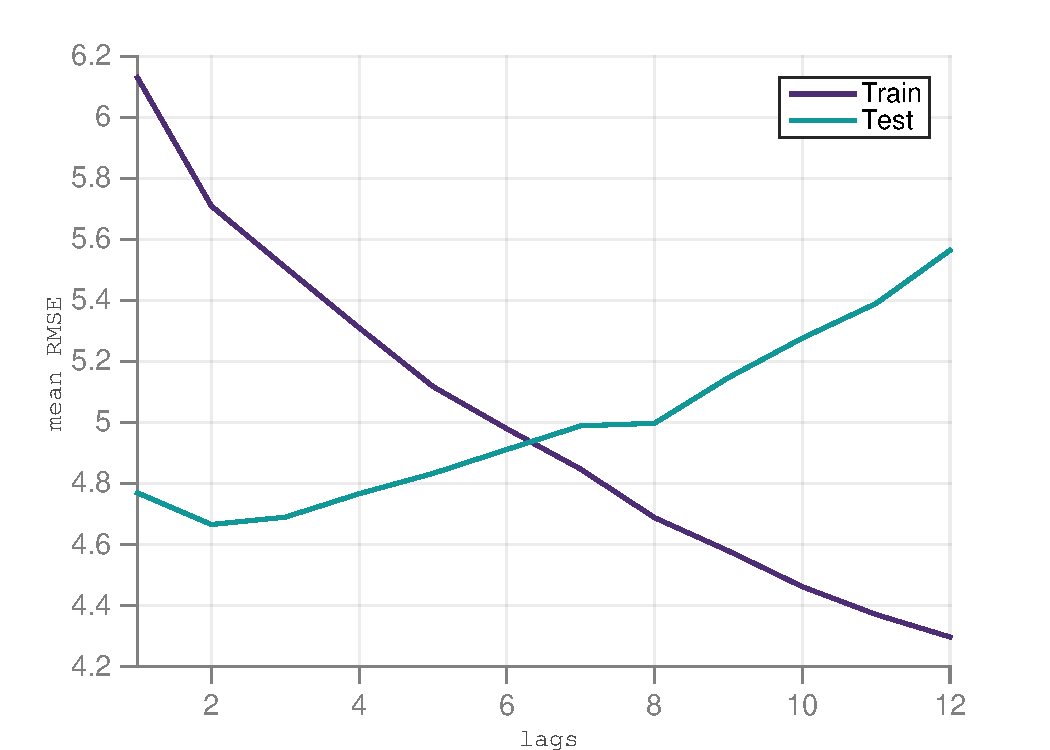
\includegraphics[width=8cm]{Figures/CVlags} &  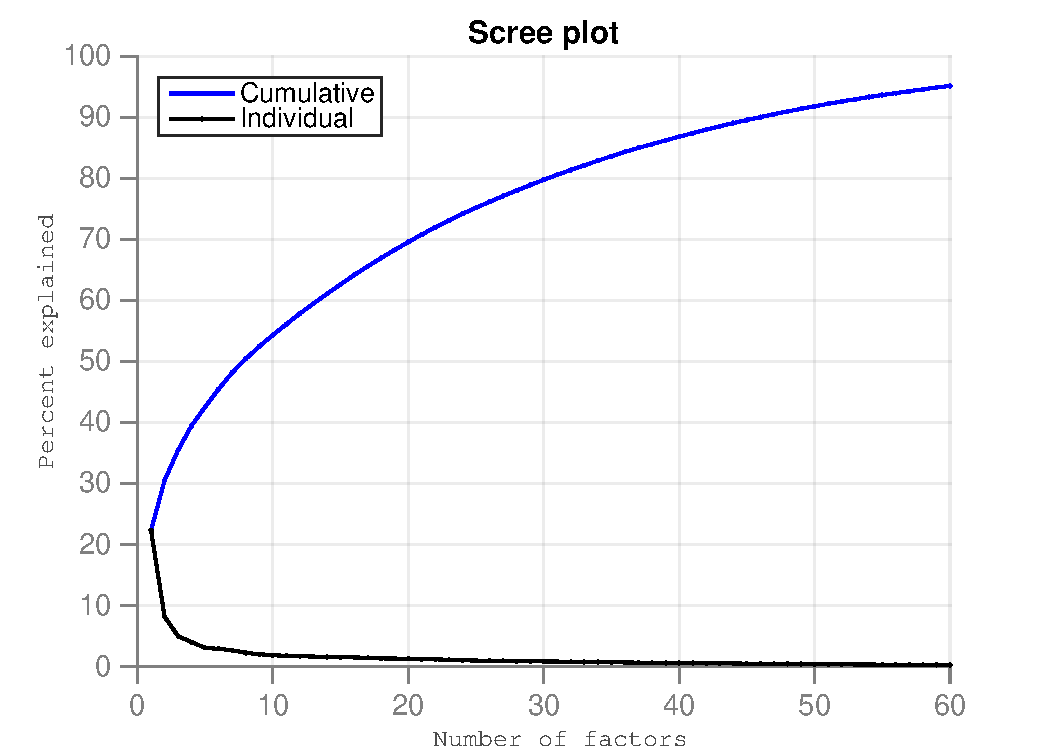
\includegraphics[width=8cm]{Figures/screeplot}
			\end{tabular}
		\end{center}
\end{figure}
		
	

\begin{figure}[H]
	\begin{center}
		\caption{\textsc{Descriptive evidence of the variables used in the SVAR}}\label{fig:descriptive}
		\begin{tabular}{cc}
			
			A. Oil price & B. Real GDP \\
			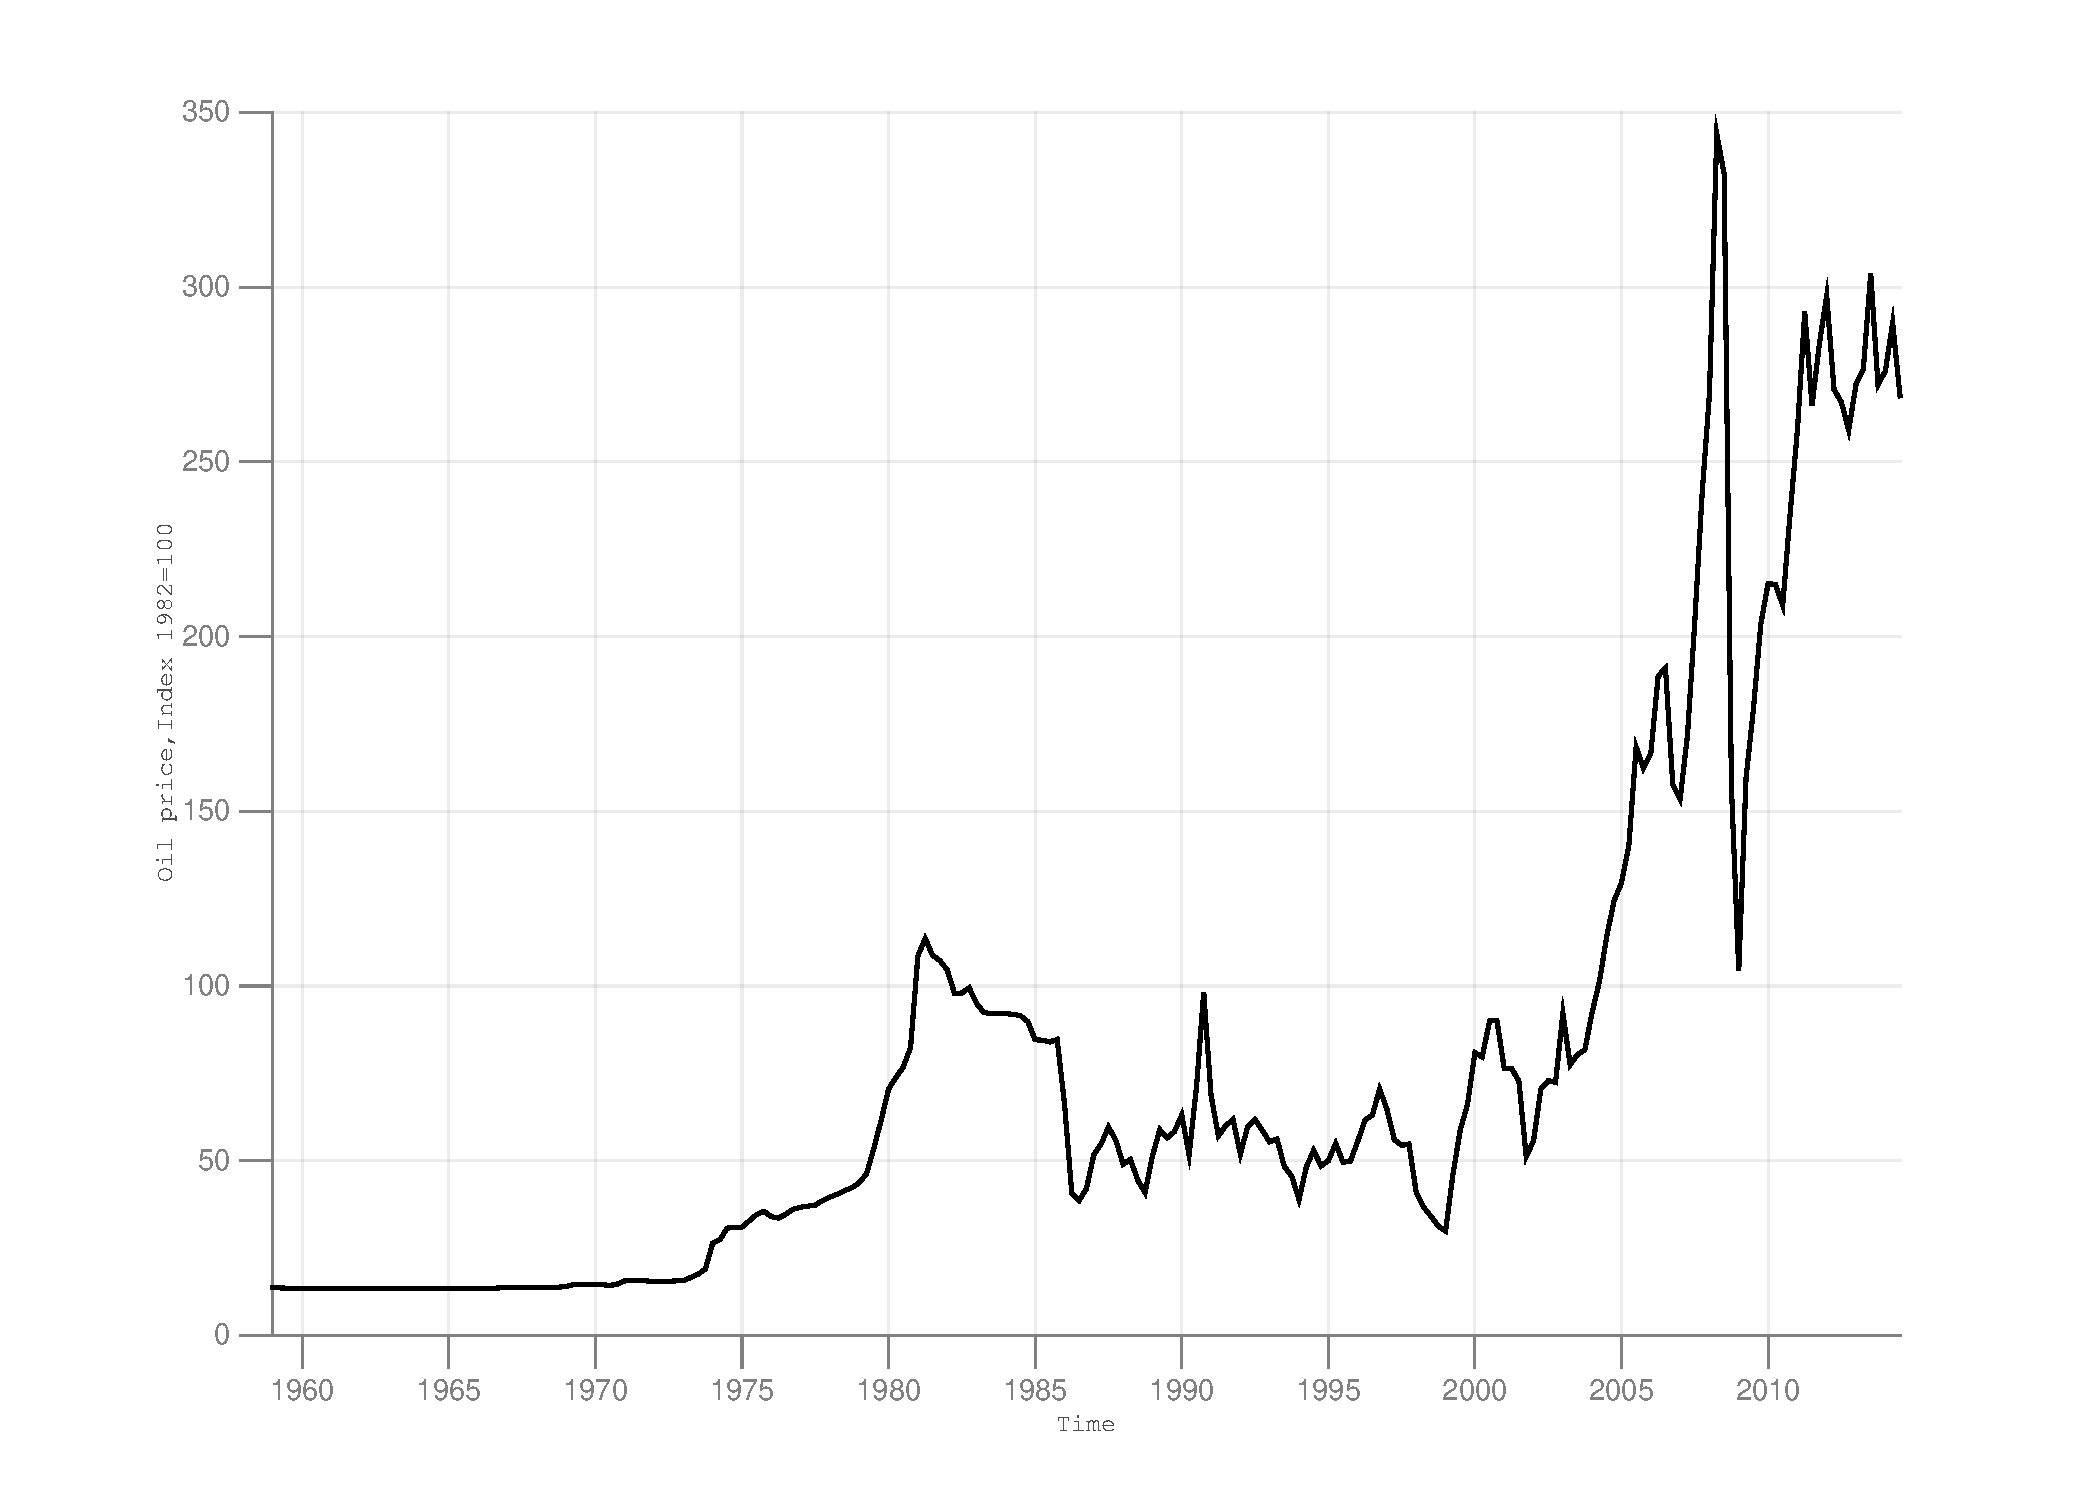
\includegraphics[width=7.5cm]{Figures/Descriptive_oil} &  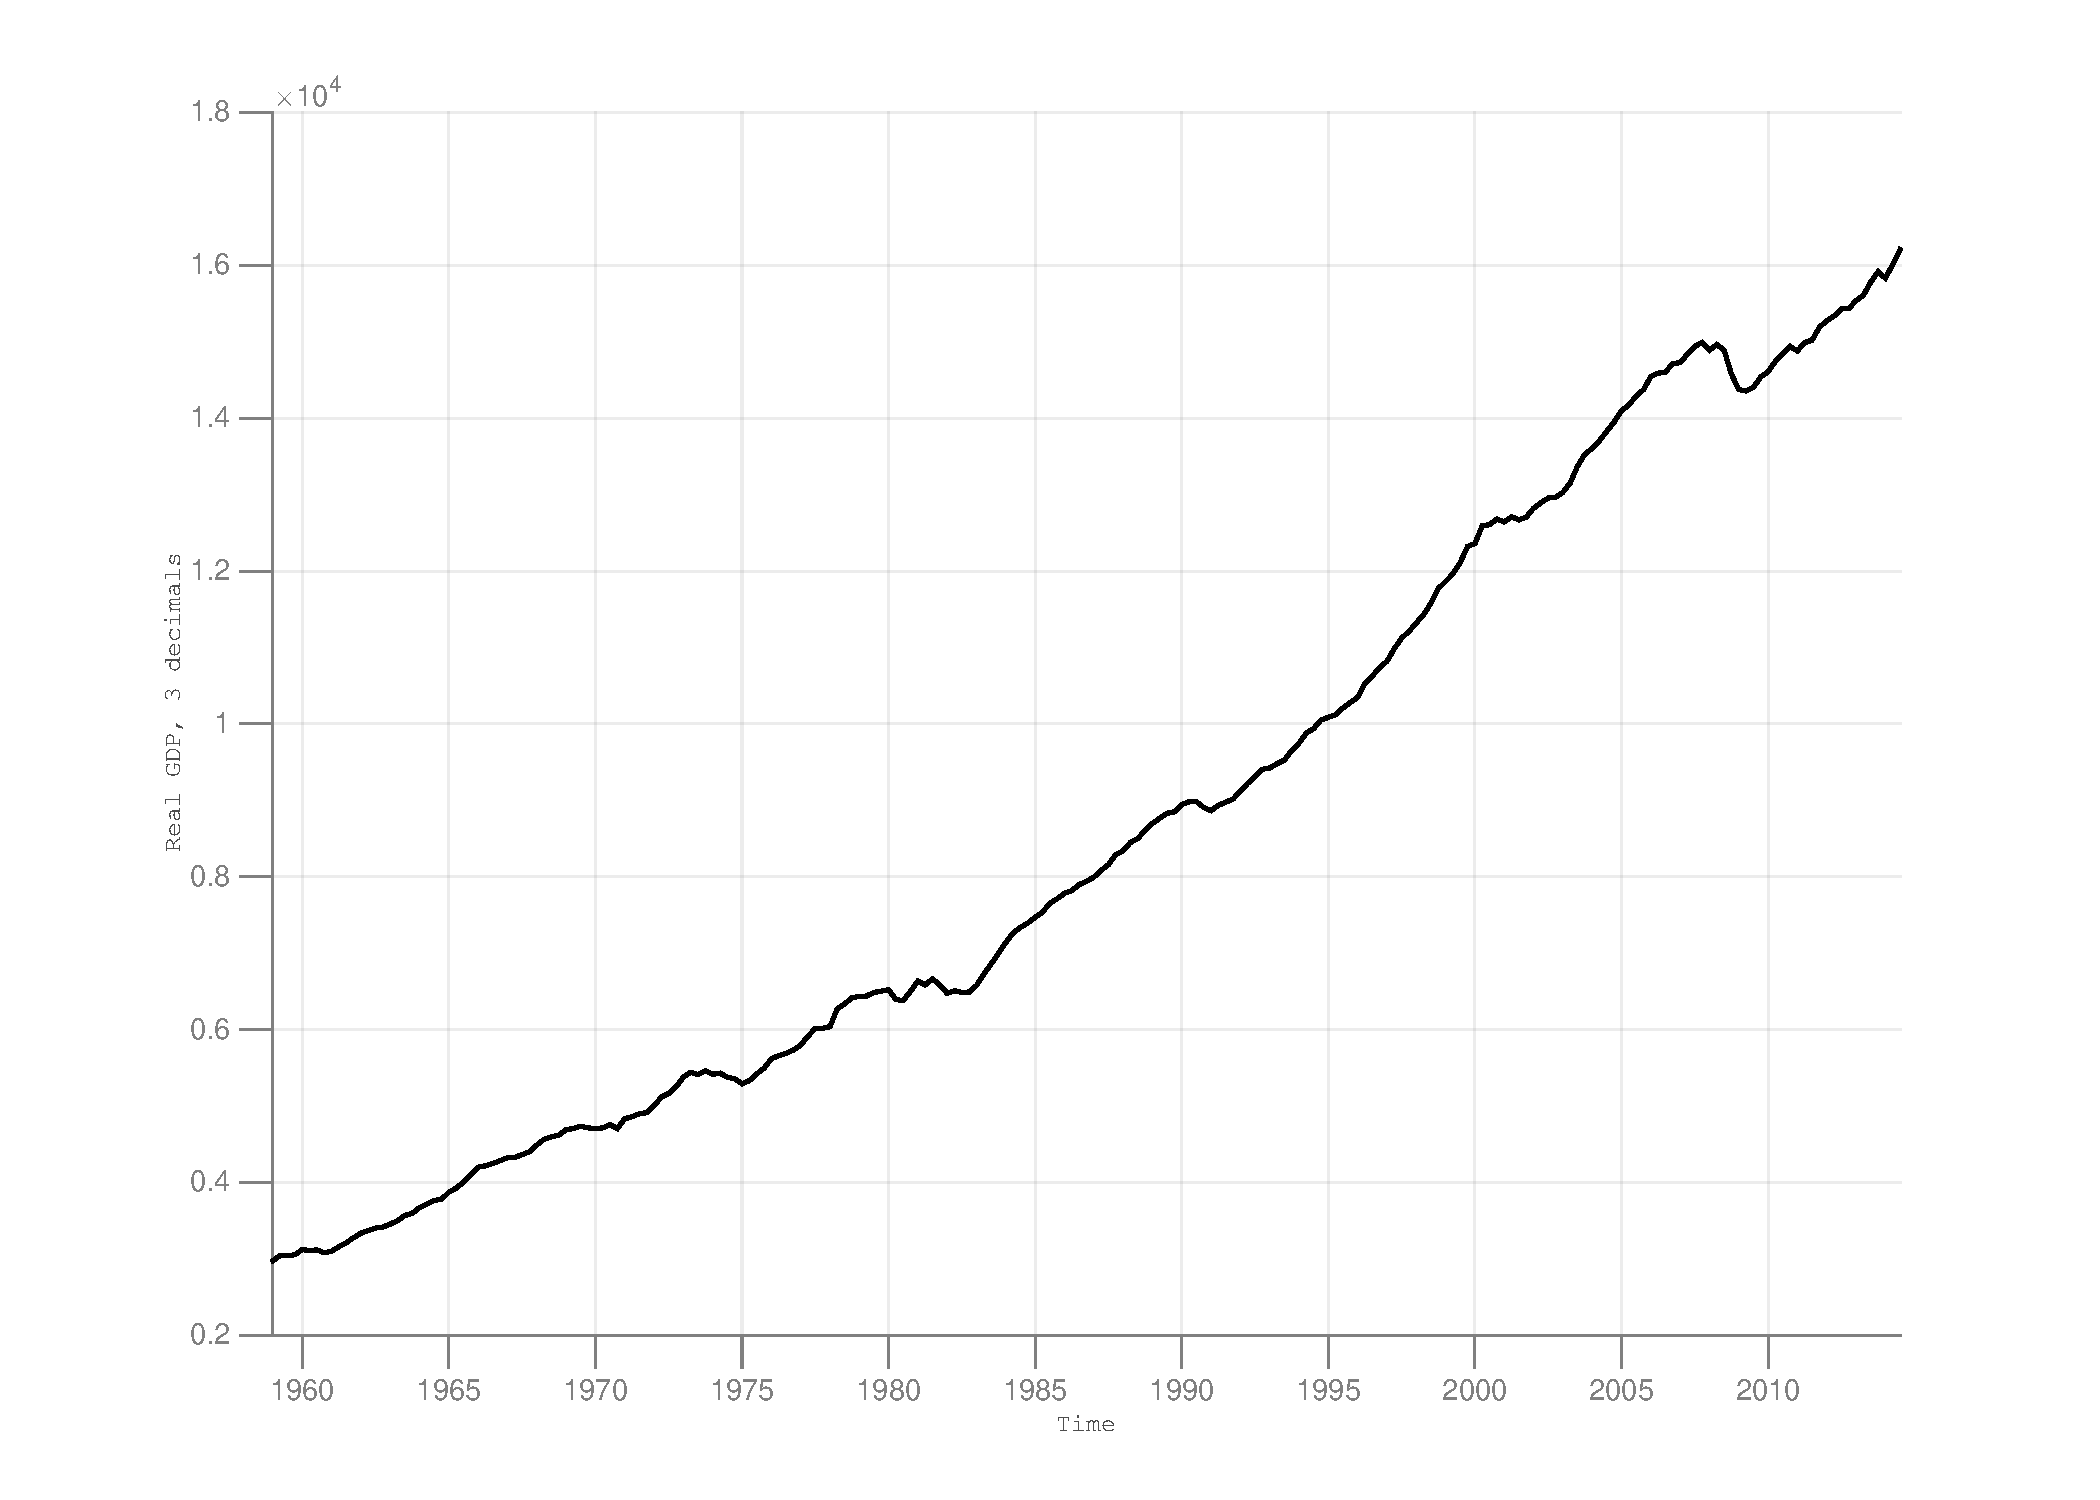
\includegraphics[width=7.5cm]{Figures/Descriptive_GDP} \\
			&\\
			C. Total Employment & D. Consumer Price Index \\
			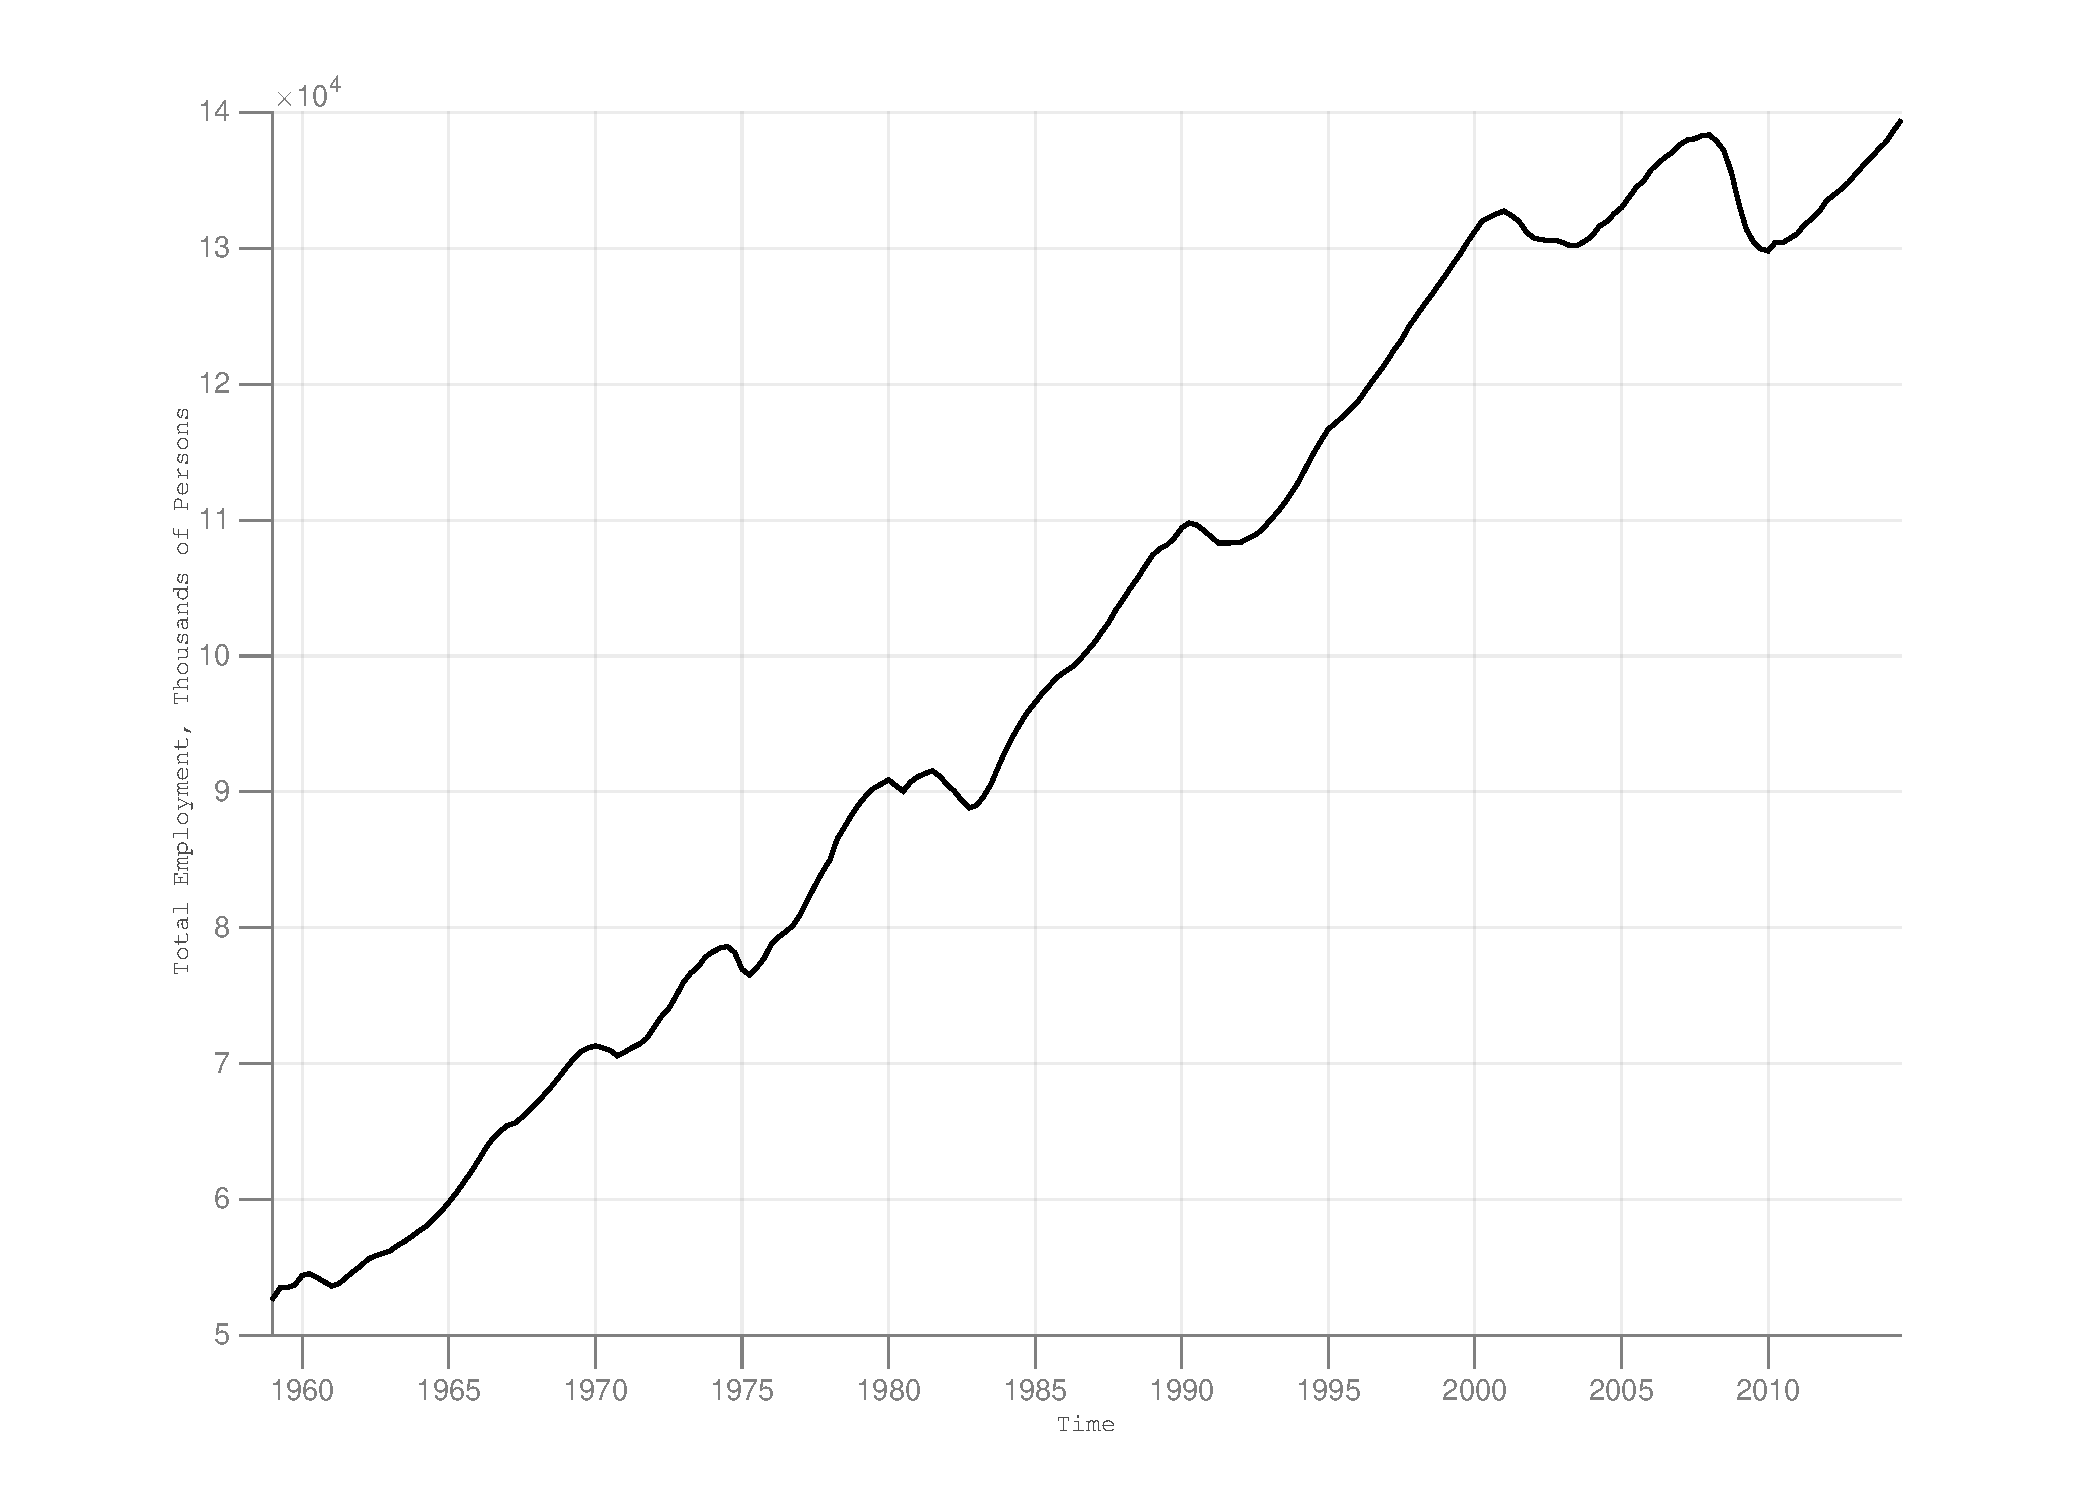
\includegraphics[width=7.5cm]{Figures/Descriptive_TOTEMP} & 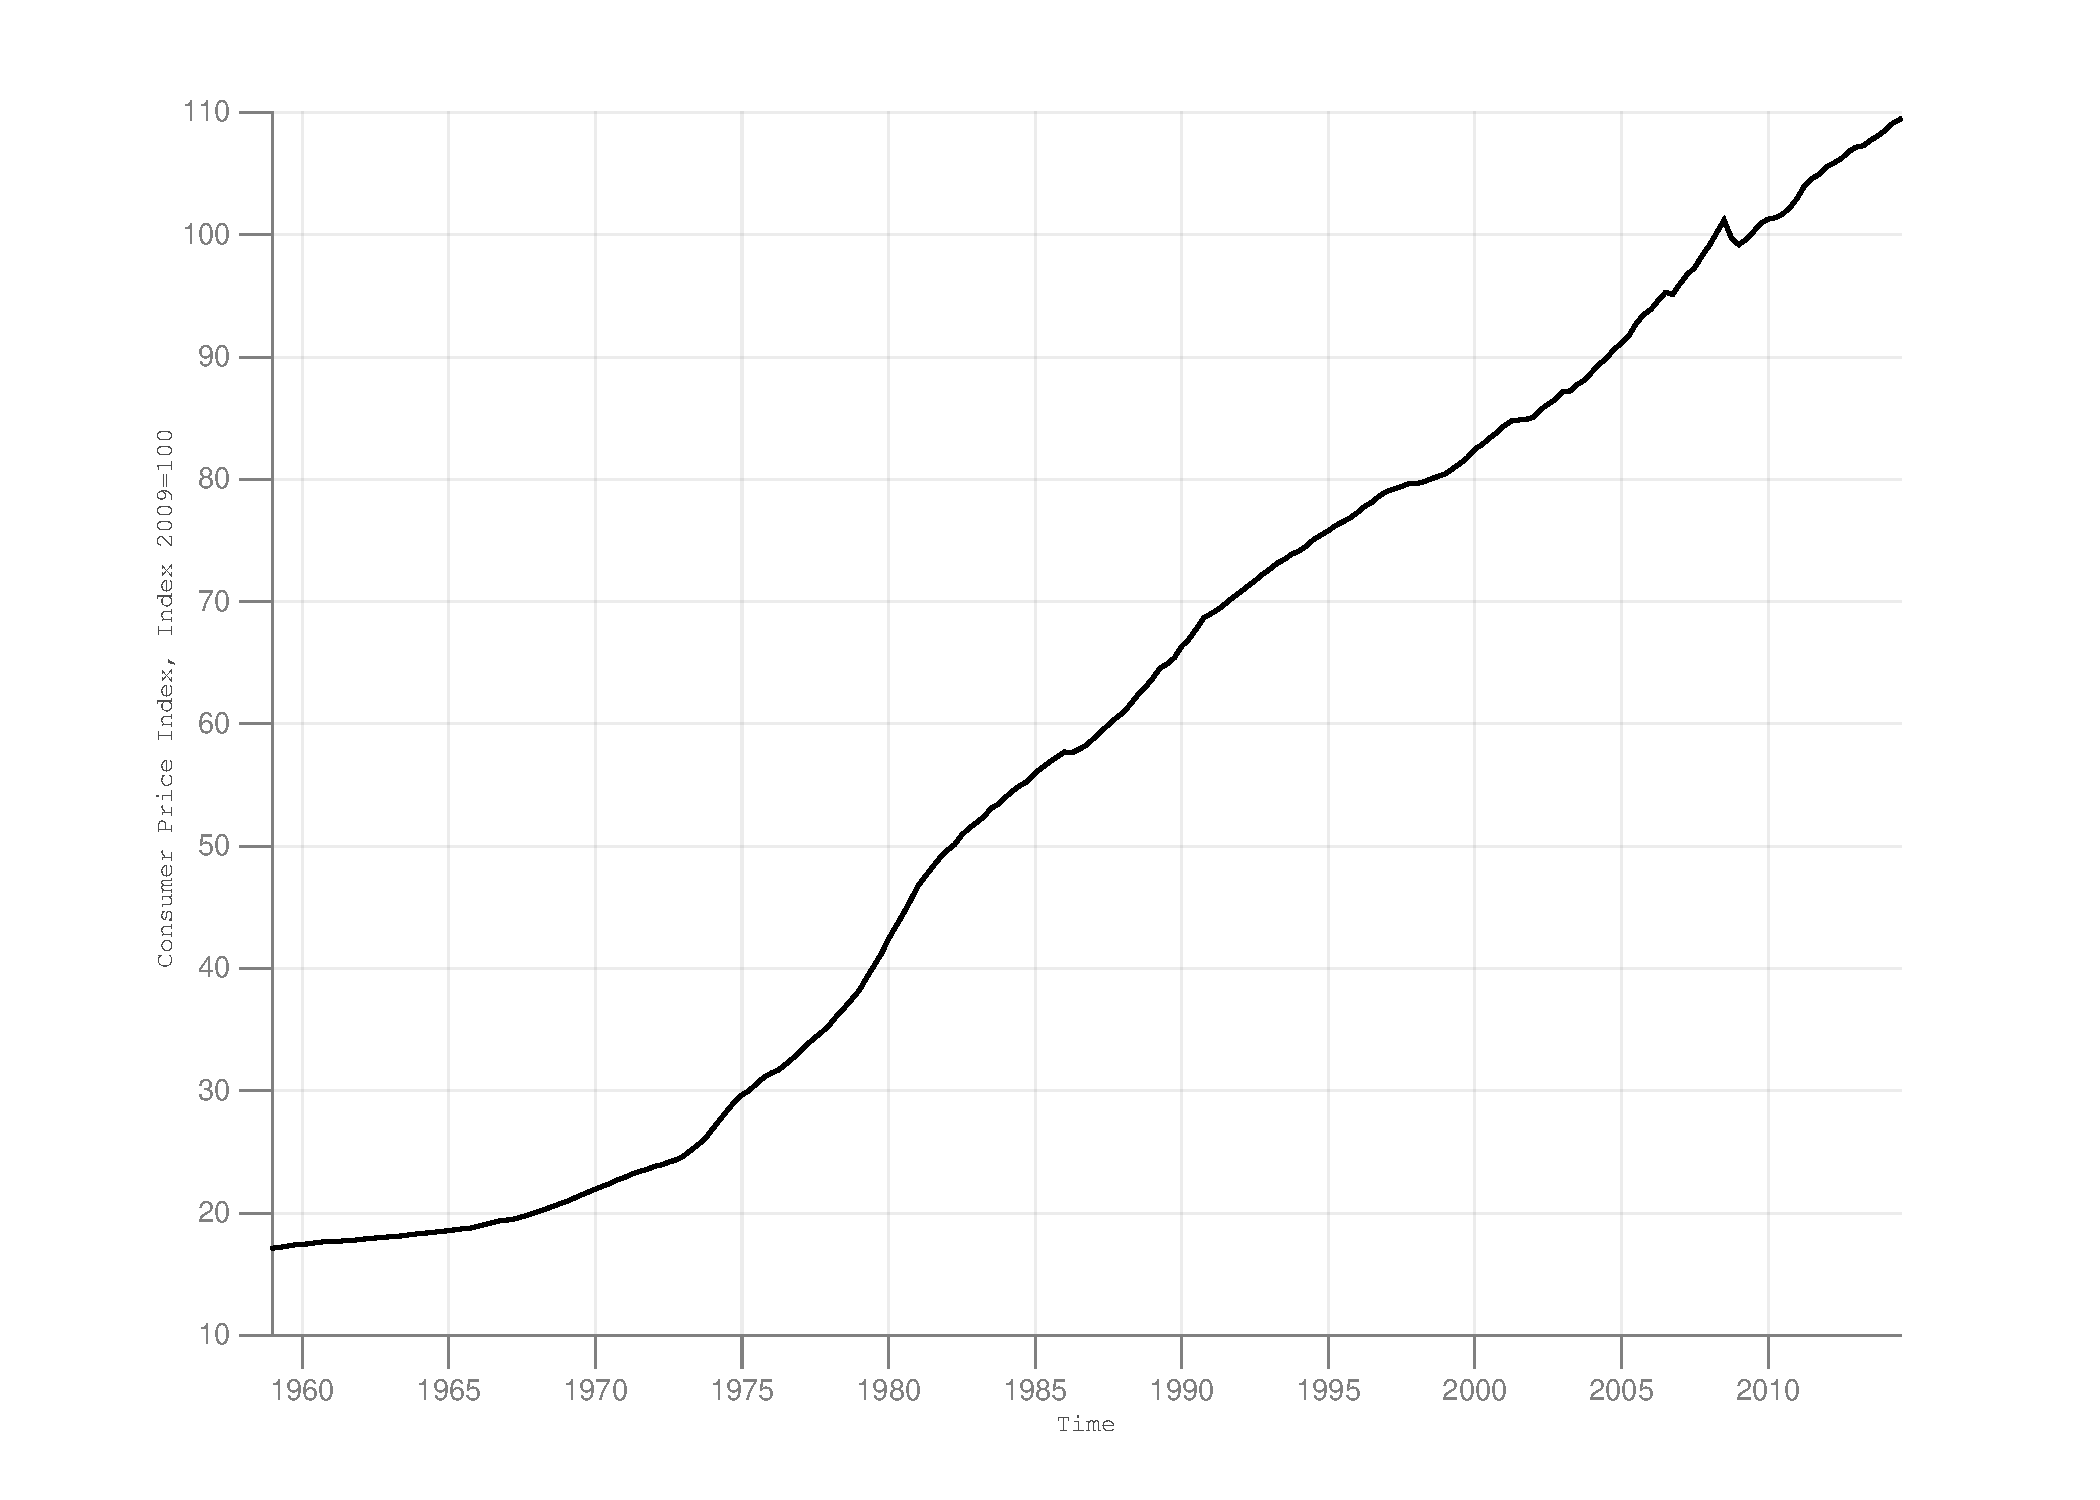
\includegraphics[width=7.5cm]{Figures/Descriptive_PCEPI} \\
			&\\
			\multicolumn{2}{c}{E. Effective Federal Funds Rate}\\
			\multicolumn{2}{c}{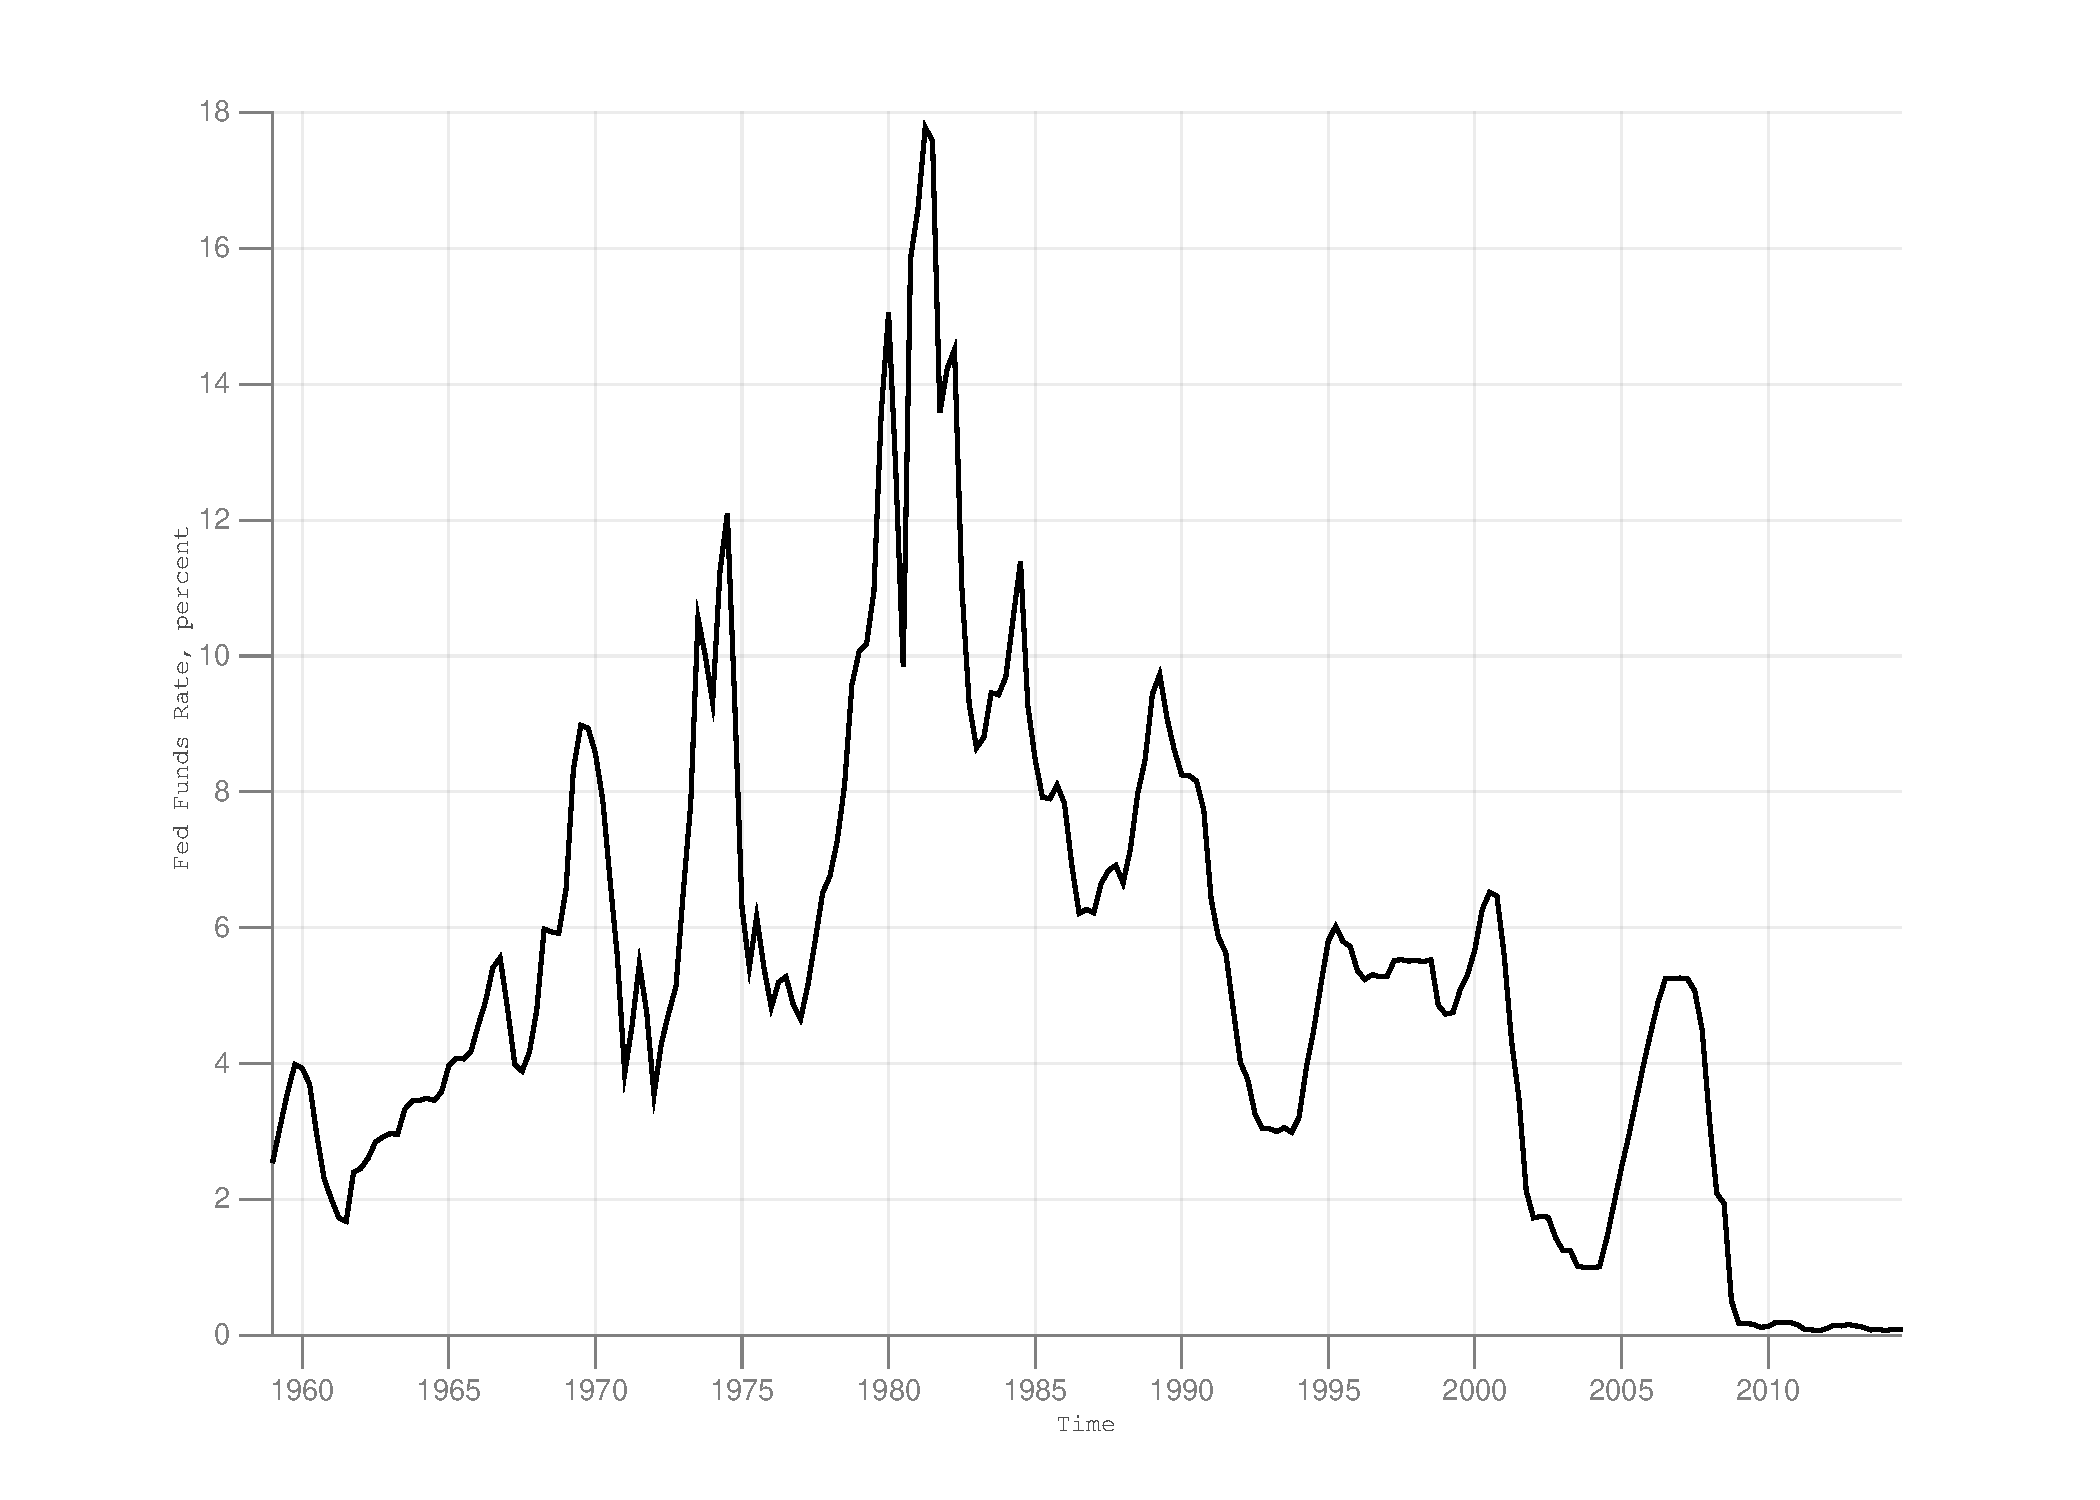
\includegraphics[width=7cm]{Figures/Descriptive_FF}}\\
		\end{tabular}
	\end{center}
		\footnotesize{\emph{Notes:  
				This figure plots the five variables included in the SVAR before any data tranformation. For detailed informations about the data see table \ref{tab:data}.}}	
\end{figure}



\begin{figure}[H]
	\begin{center}
		\caption{\textsc{Structural impulse response functions from the SVAR}}
		\label{fig:SVAR_irf}
		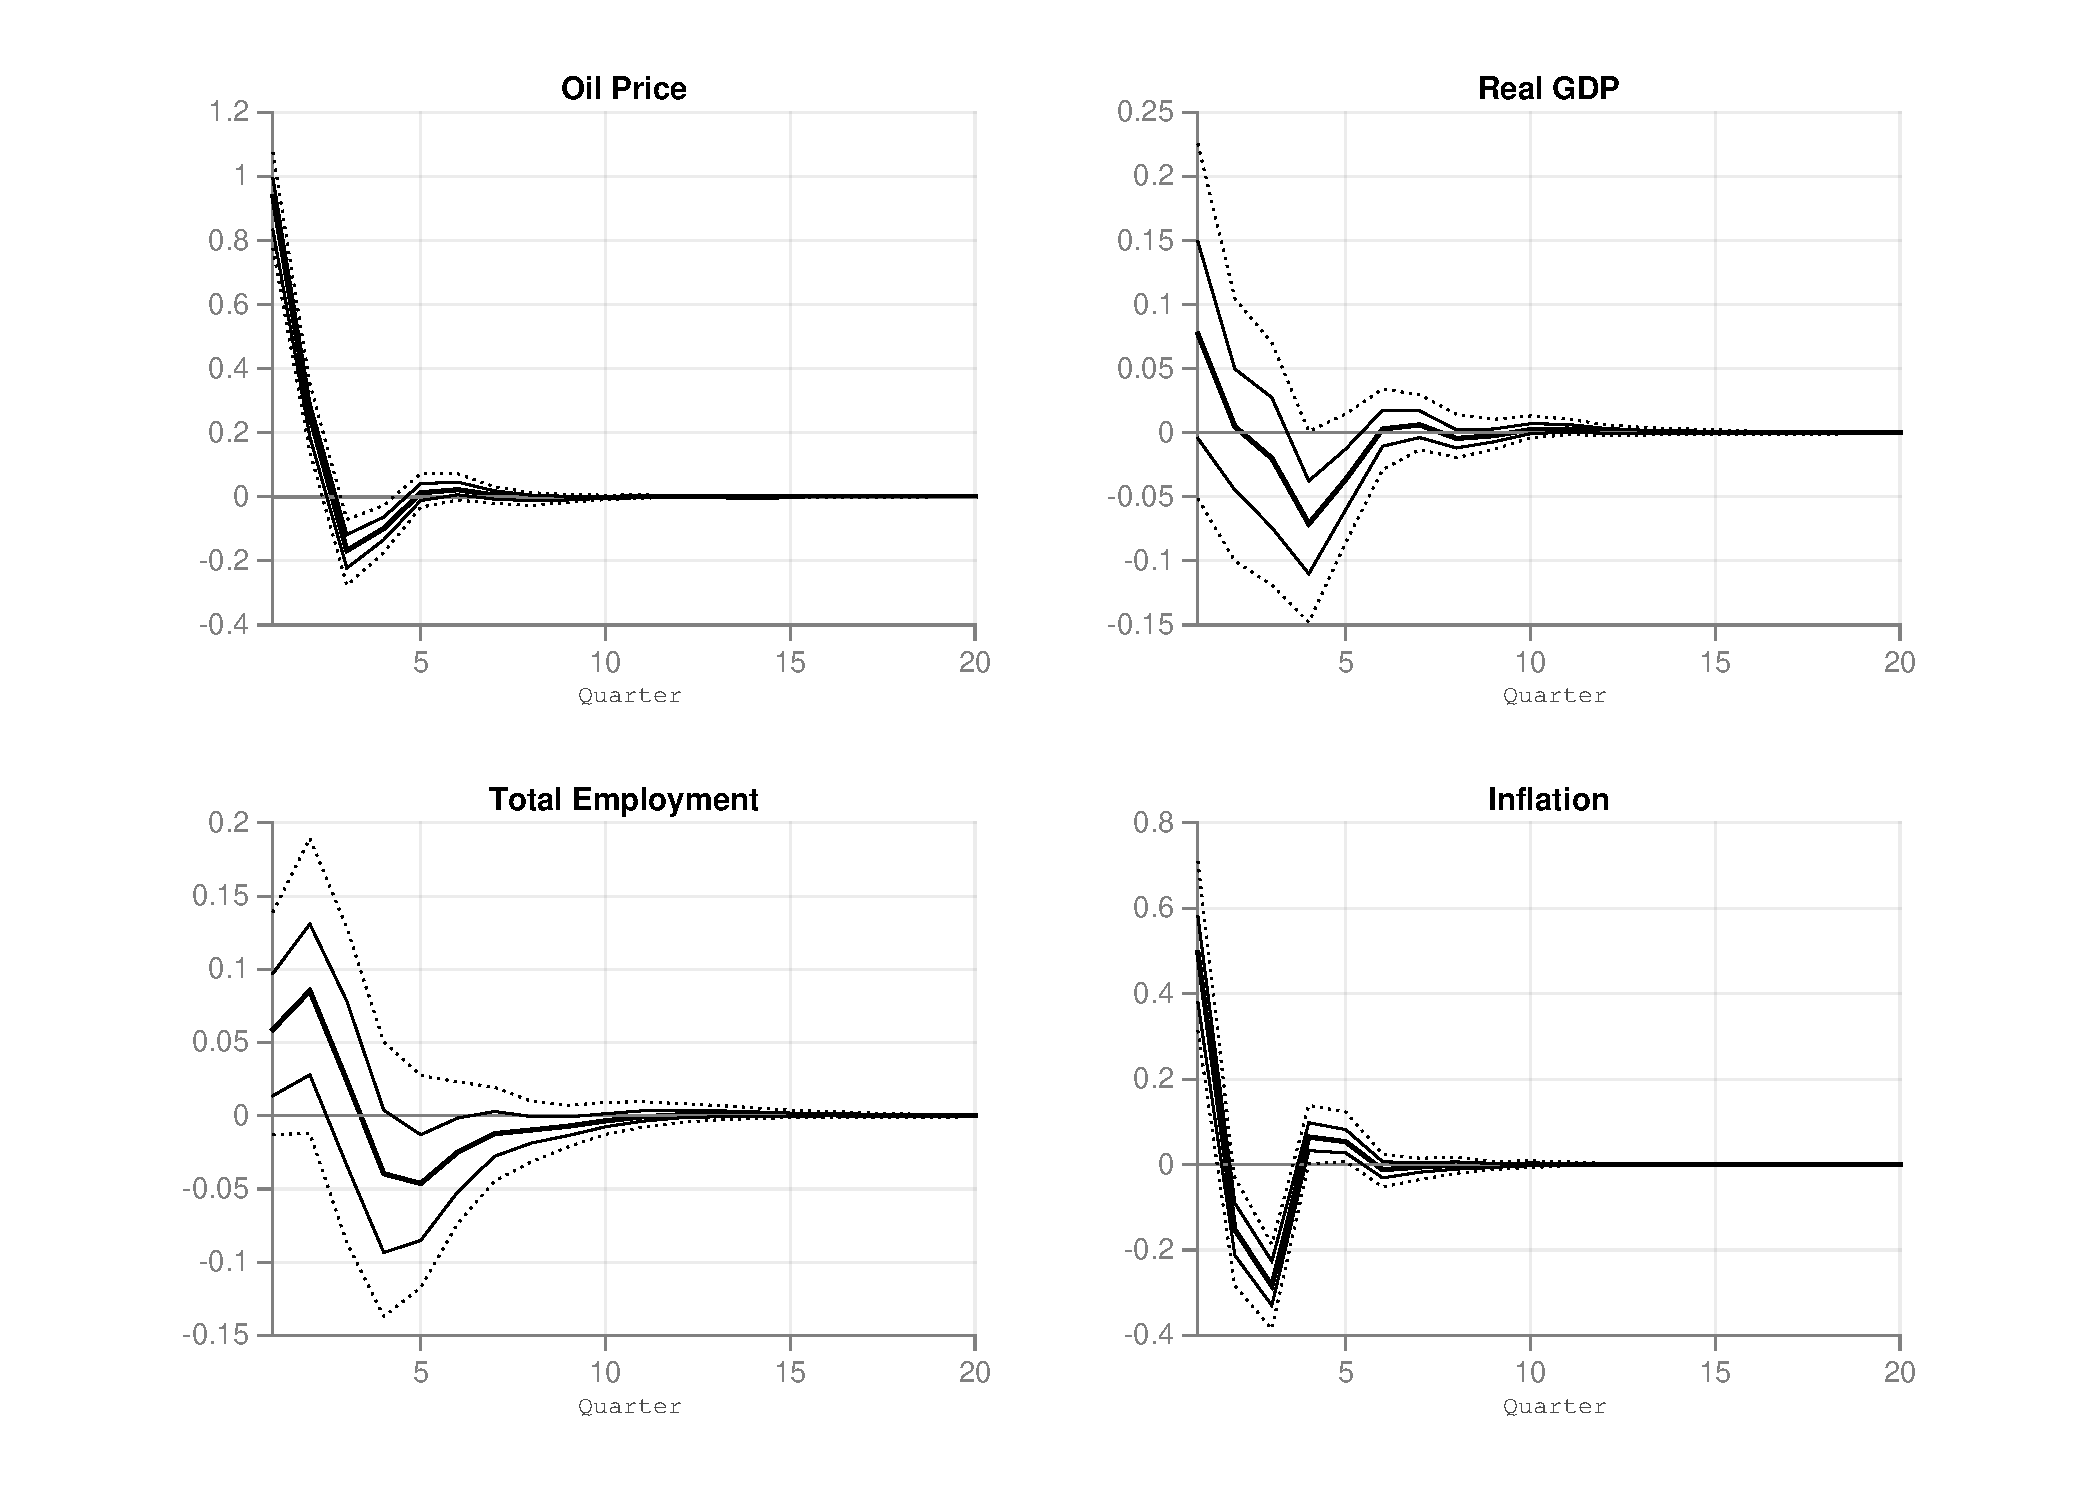
\includegraphics[width=0.5\textheight]{Figures/SVAR_irf}
	\end{center}
	\footnotesize{\emph{Notes:
			This figure presents structural impulse response functions from the SVAR (black solid line with 60\% and 90\% standard error bands) with respect to an oil price shock. 
			The variables included are:  growth rate of  oil price,  growth rate of real GDP,  growth rate of total employment,  change in inflation and  change in interest rate.
			We identify this structural shock by ranking oil price first the the SVAR. The order the subsequent variables has no importance with respect to identifying the structural impulse response functions for an oil price shock.  }
	}
\end{figure}




\begin{figure}[H]
	\begin{center}
		\caption{\textsc{Structural impulse response functions from the FAVAR}}
		\label{fig:FAVAR_irf}
		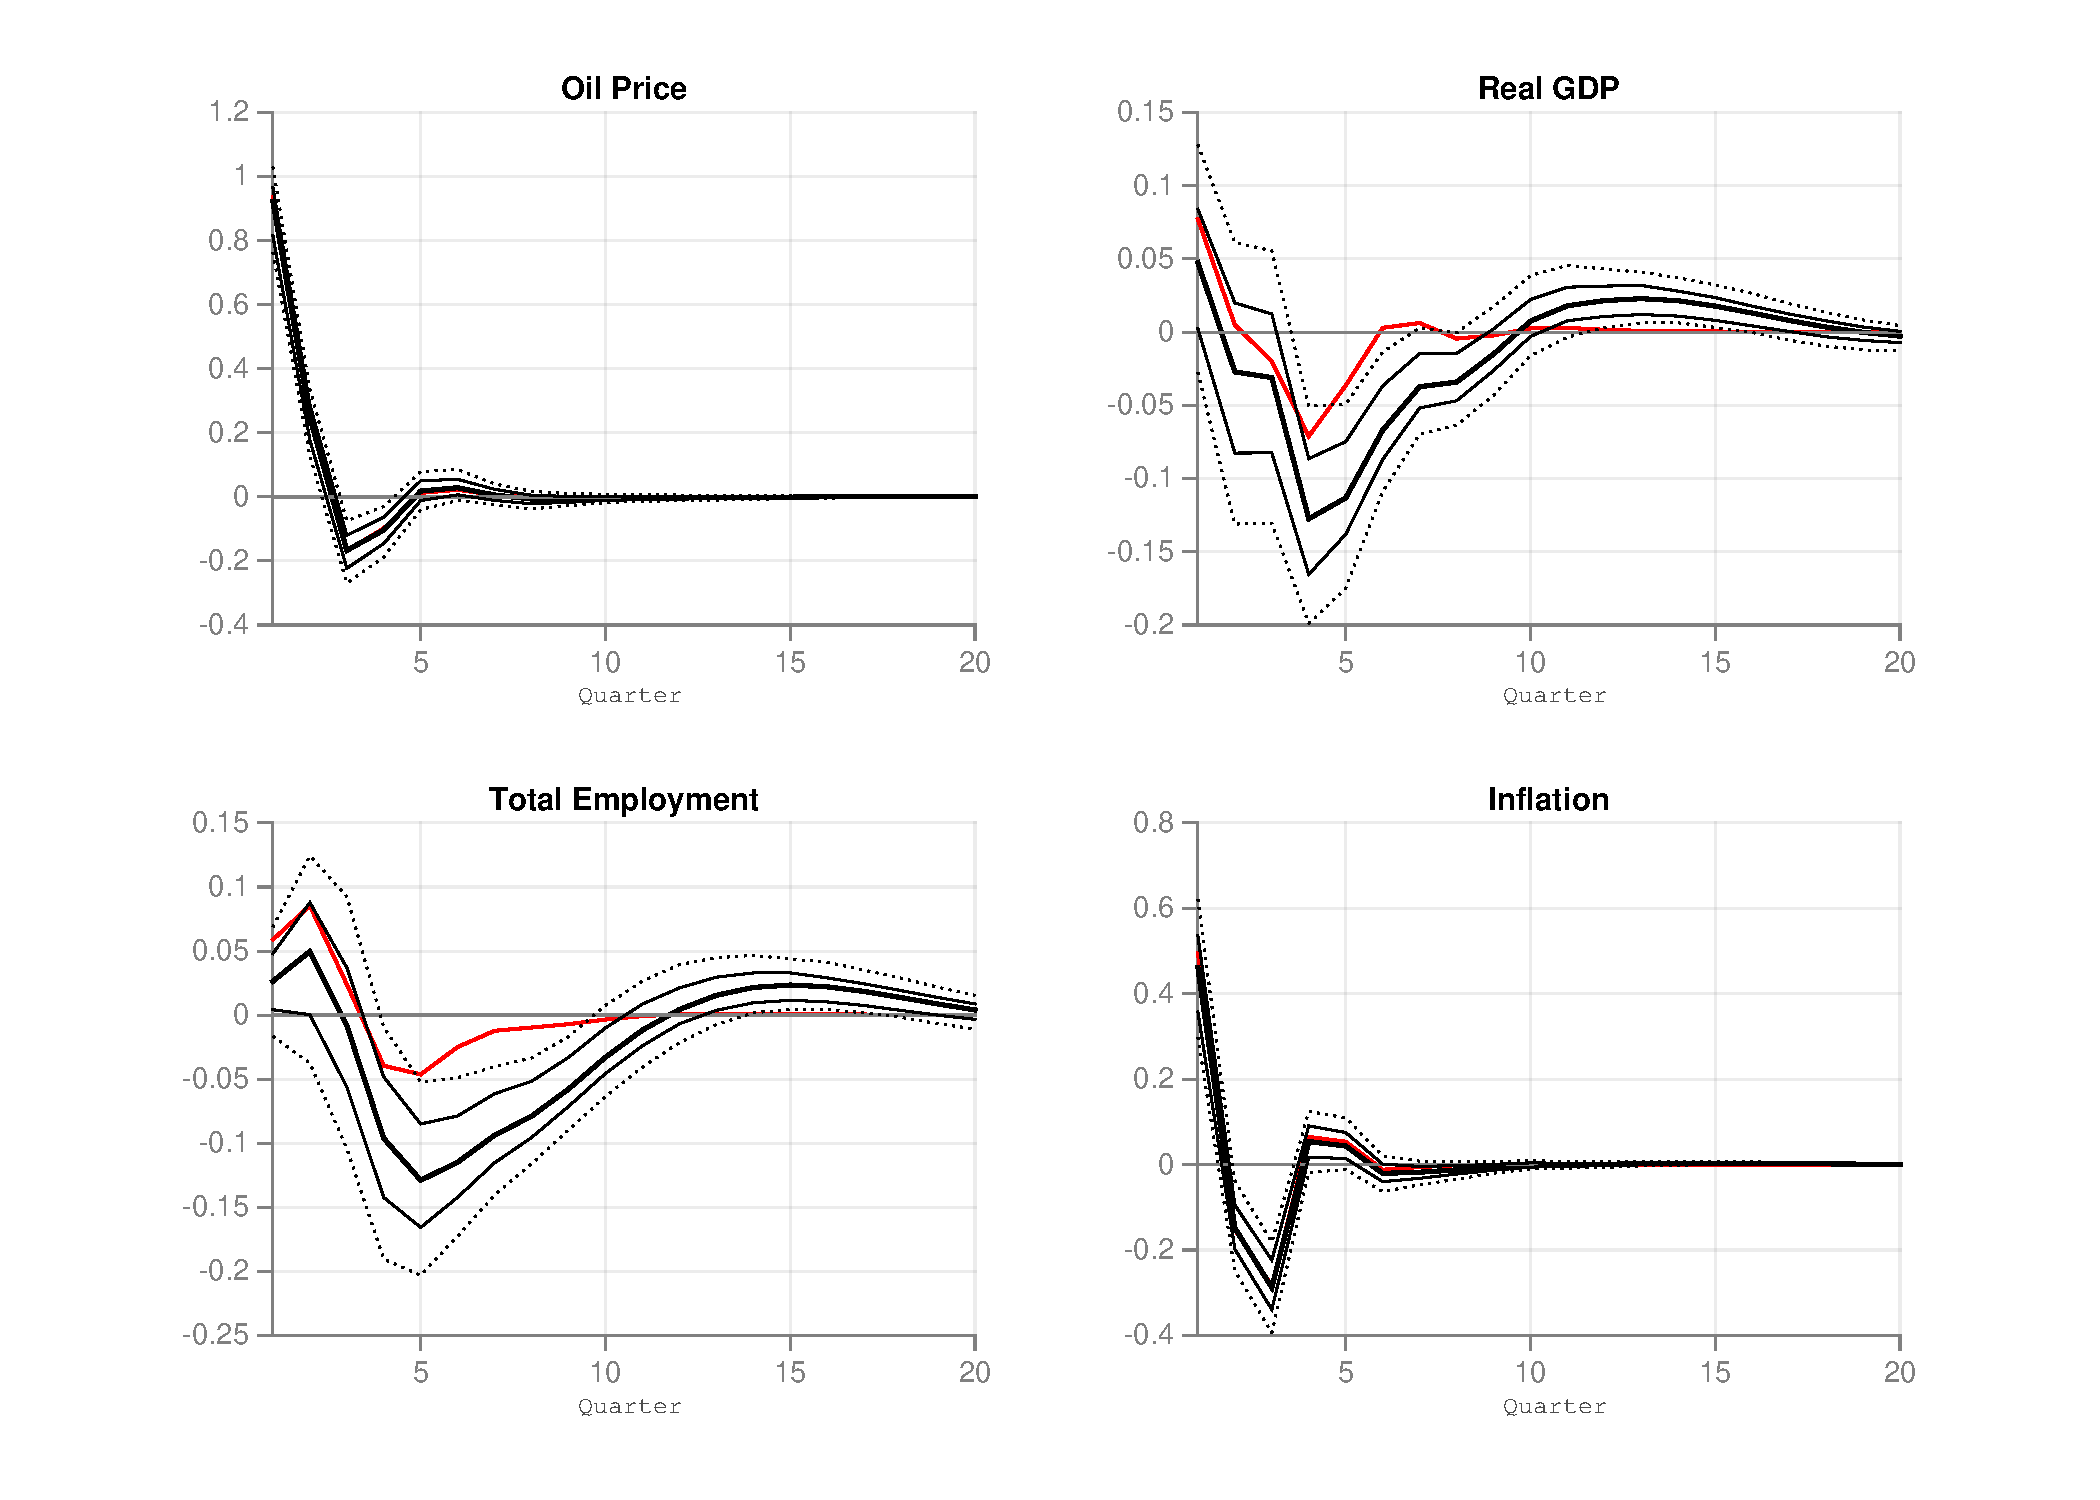
\includegraphics[width=0.5\textheight]{Figures/FAVAR_irf}
	\end{center}
	\footnotesize{\emph{Notes:
			This figure presents structural impulse response functions from the FAVAR (black solid line with 60\% and 90\% standard error bands) and the SVAR (red solid line, see figure \ref{fig:SVAR_irf}) with respect to an oil price shock. We construct the FAVAR by augmenting the initial SVAR with two factors computed using principal component analysis from a data set of 106 variables describing the US economy. We identify this structural shock by ranking oil price first the FAVAR.}
	}
\end{figure}



\newpage

\begin{landscape}
	\begin{figure}[H]
		\begin{center}
			\caption{\textsc{Robustness checks}}
			\label{fig:robustness}
			\begin{tabular}{ccc}
				A. Before the Great Moderation & B. After the Great Moderation & C. Without the ZLB period \\
				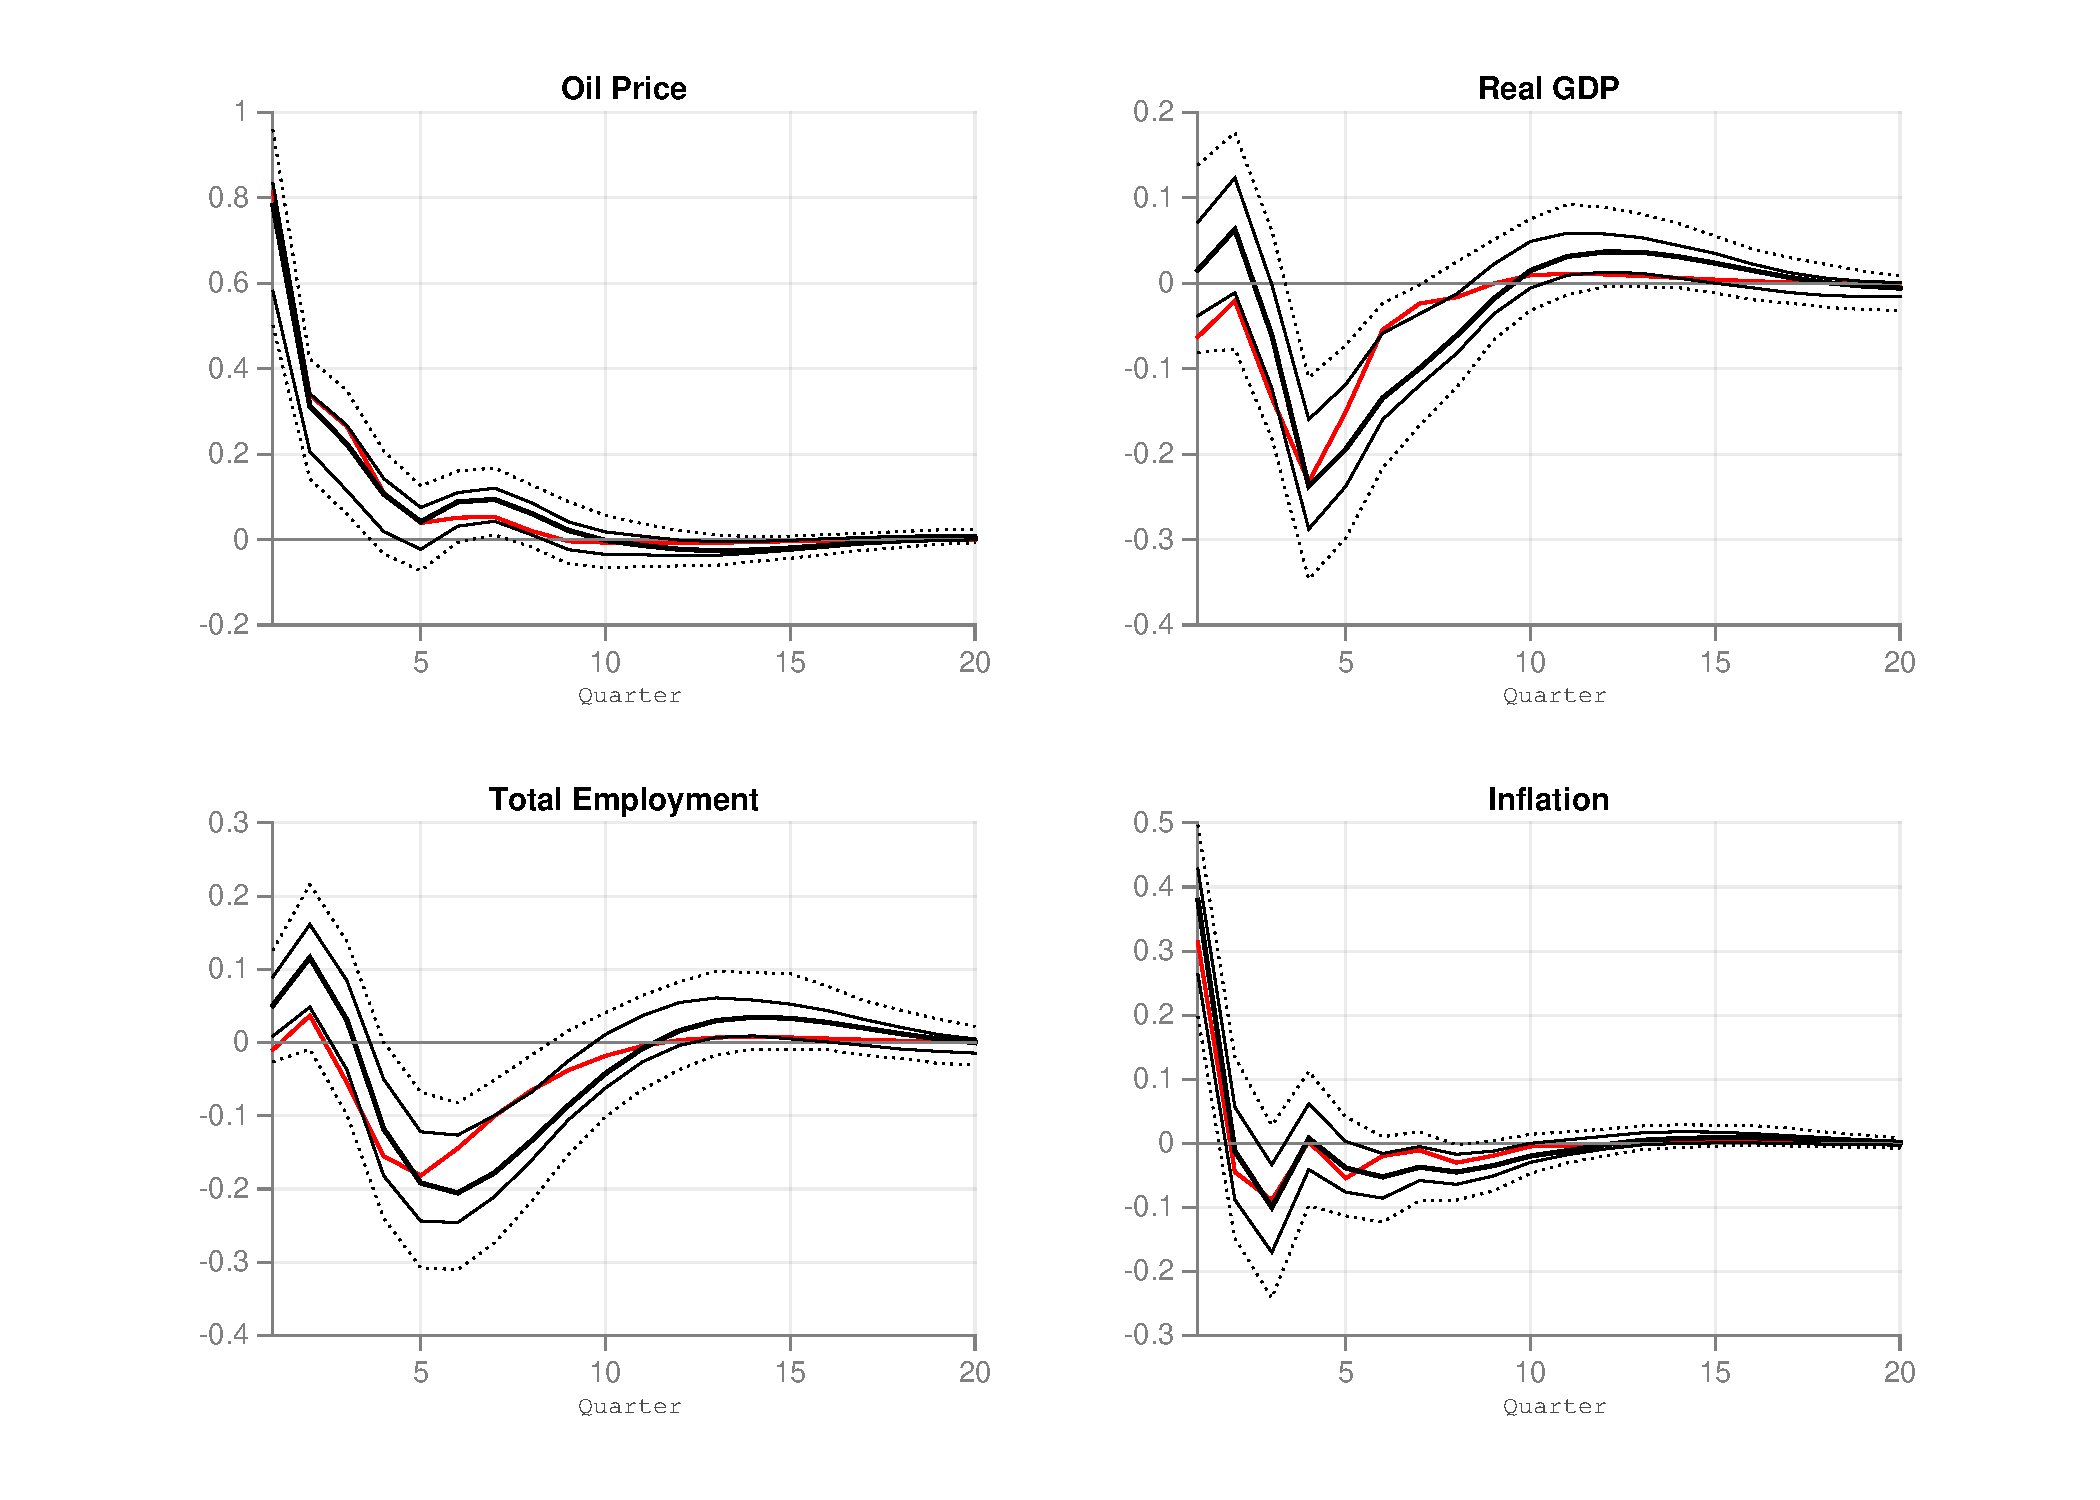
\includegraphics[width=7.5cm]{Figures/Robustness_beforeGM} &  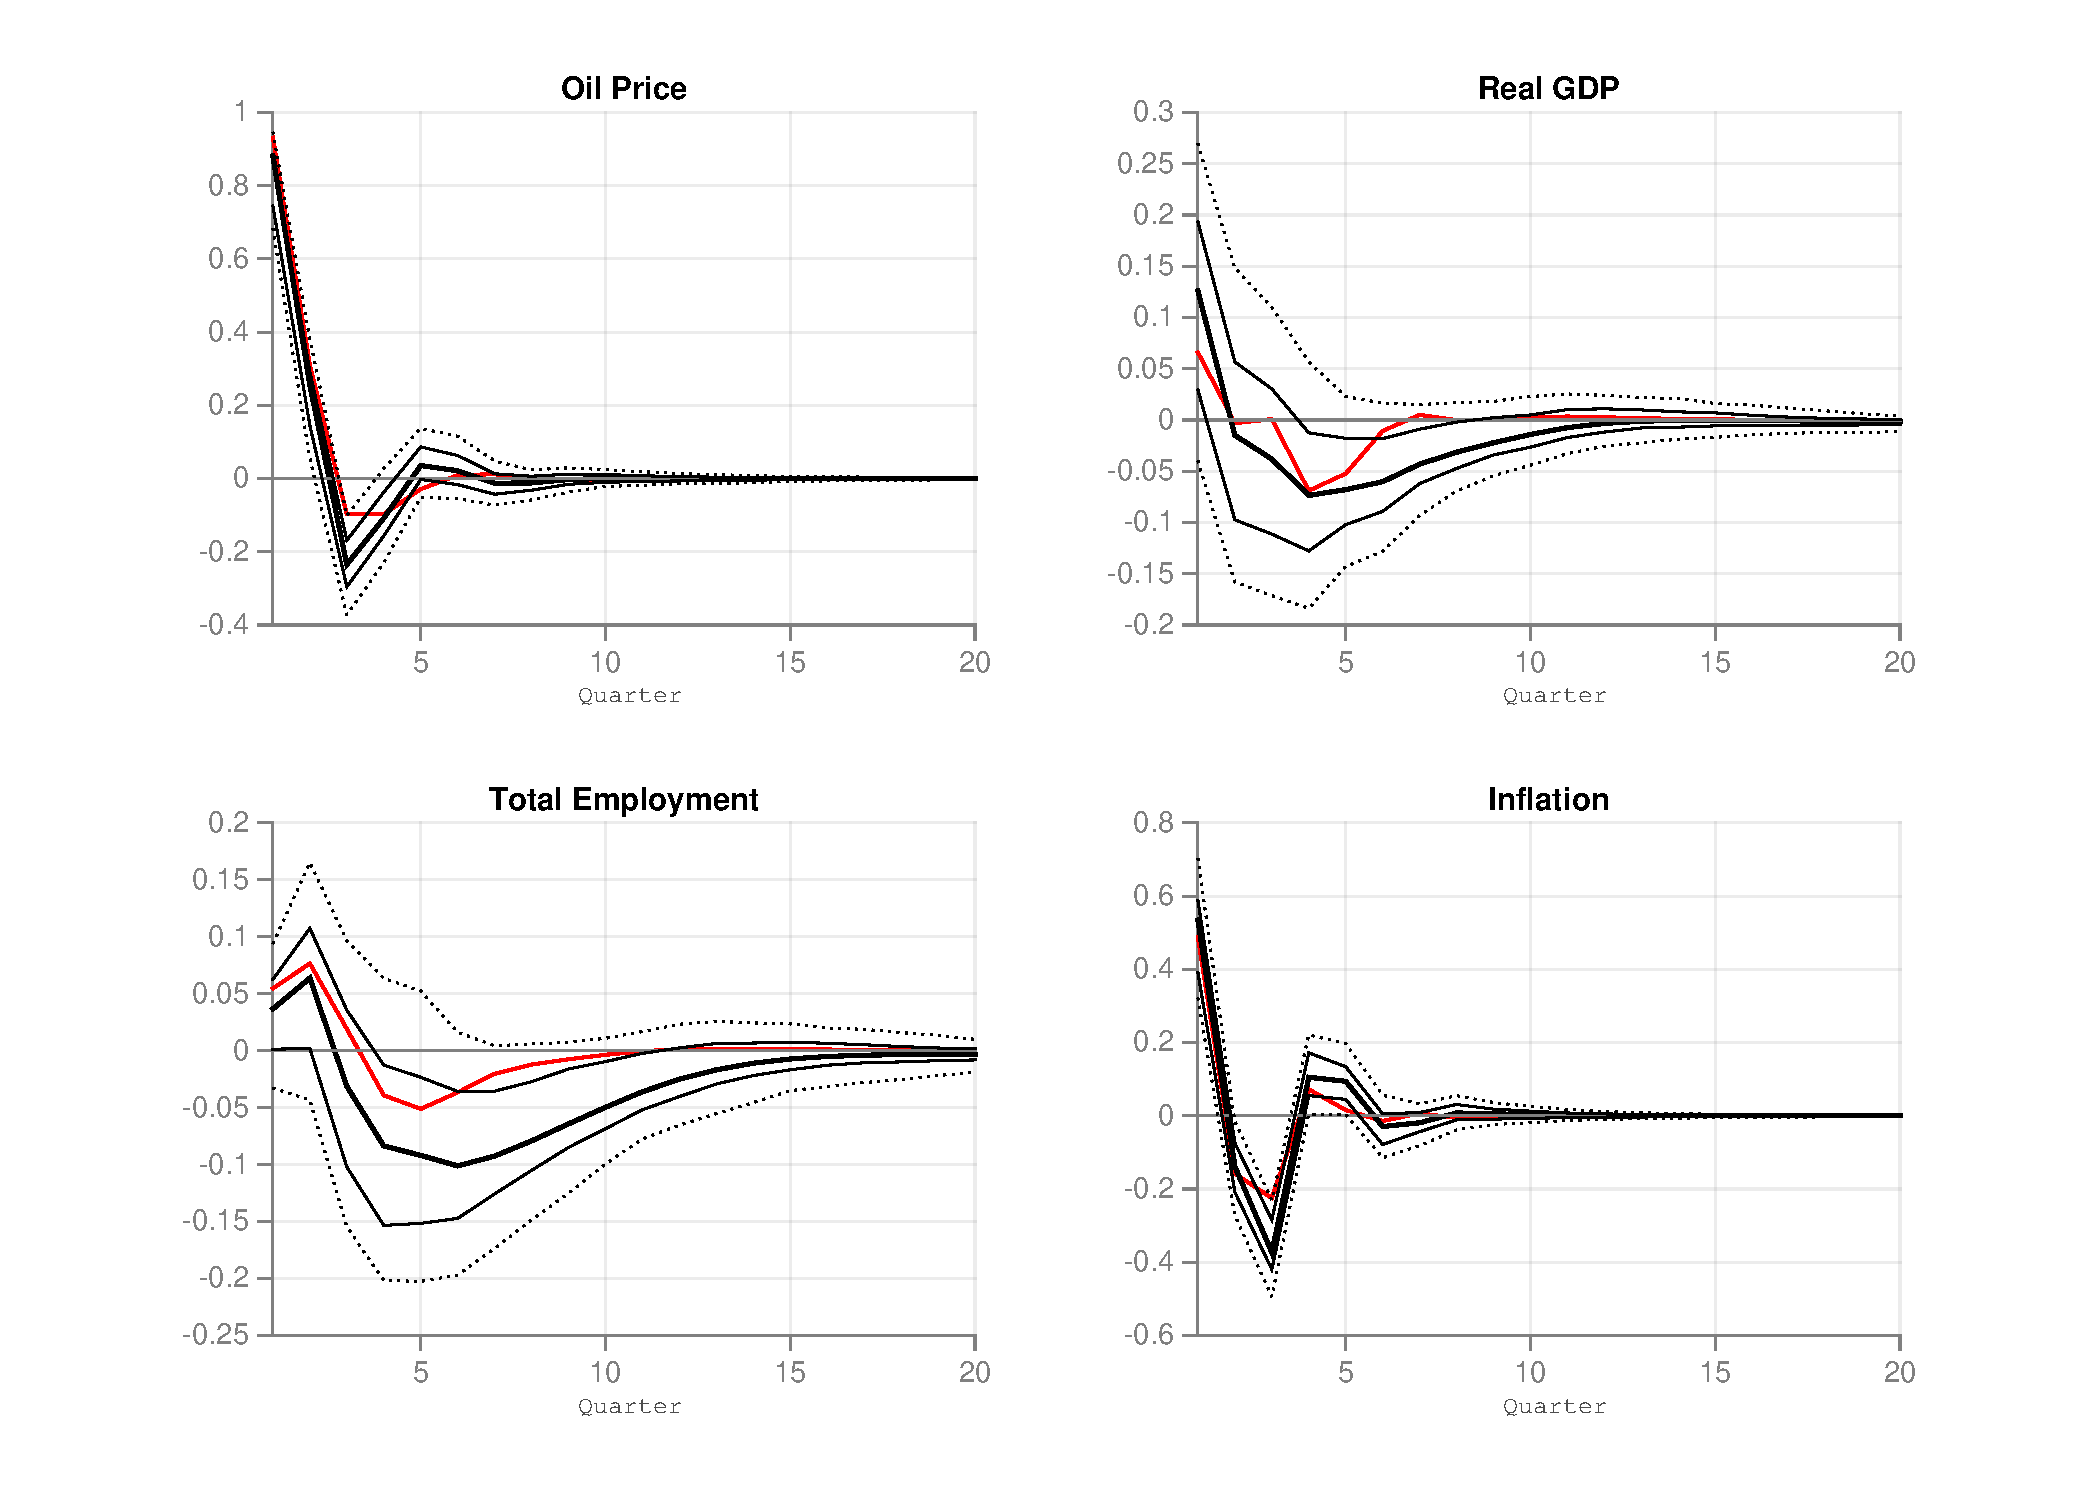
\includegraphics[width=7.5cm]{Figures/Robustness_afterGM}&
				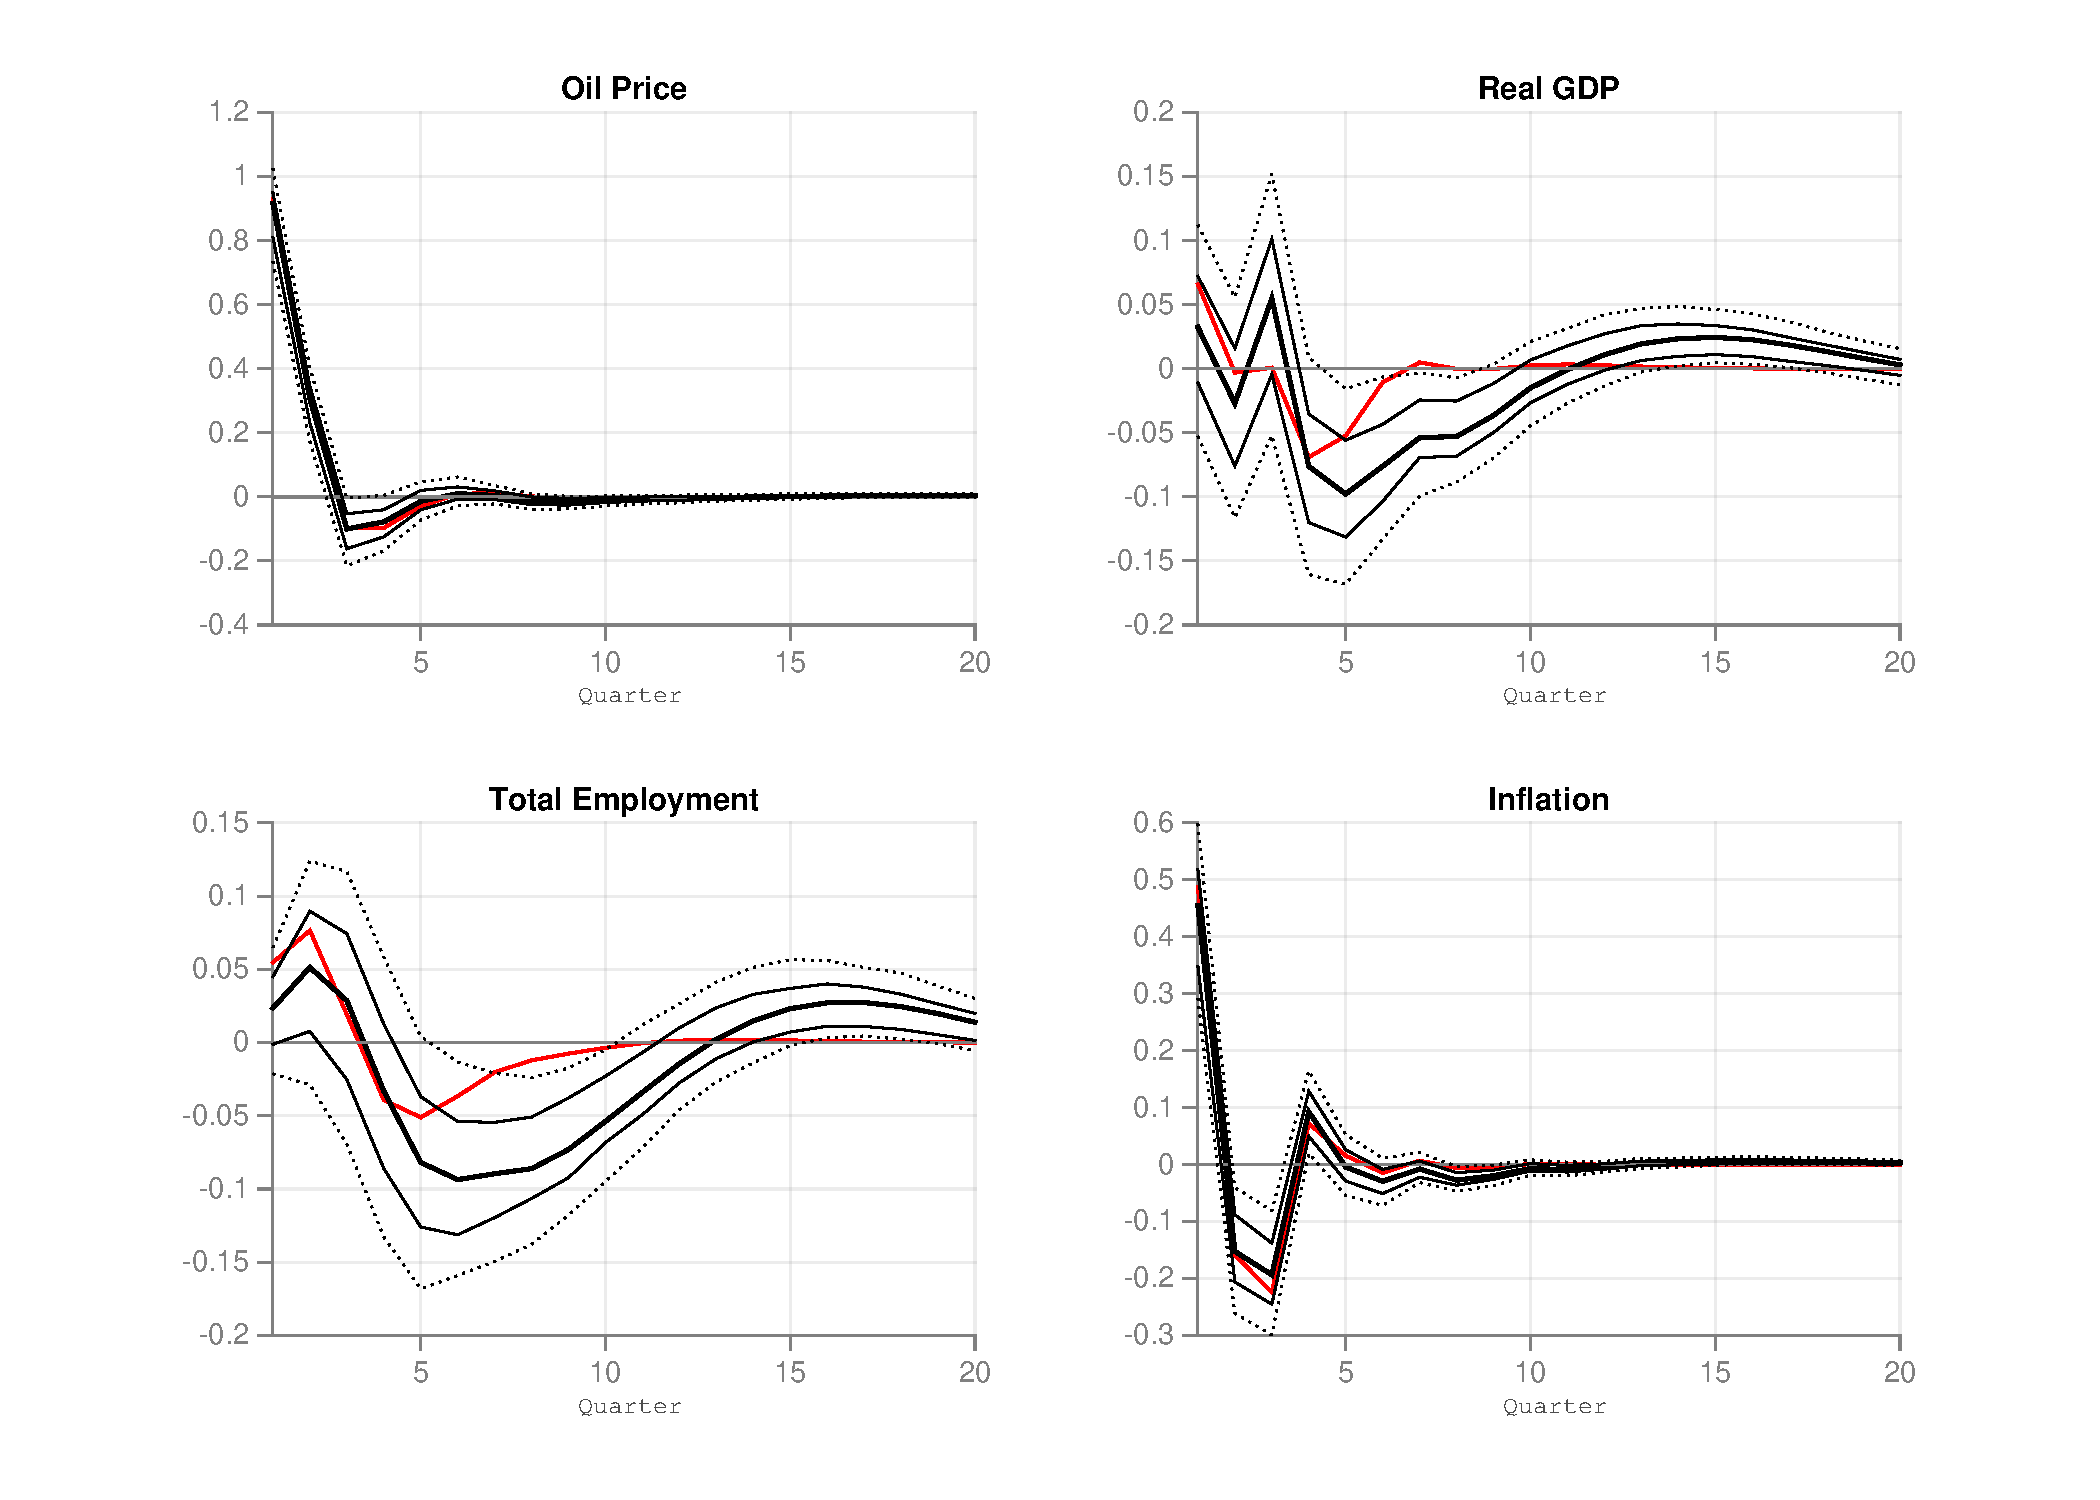
\includegraphics[width=7.5cm]{Figures/Robustness_ZLB} \\
				D. Using 3 Lags  & E. Using 8 Lags & F. Using 3 Factors  \\
				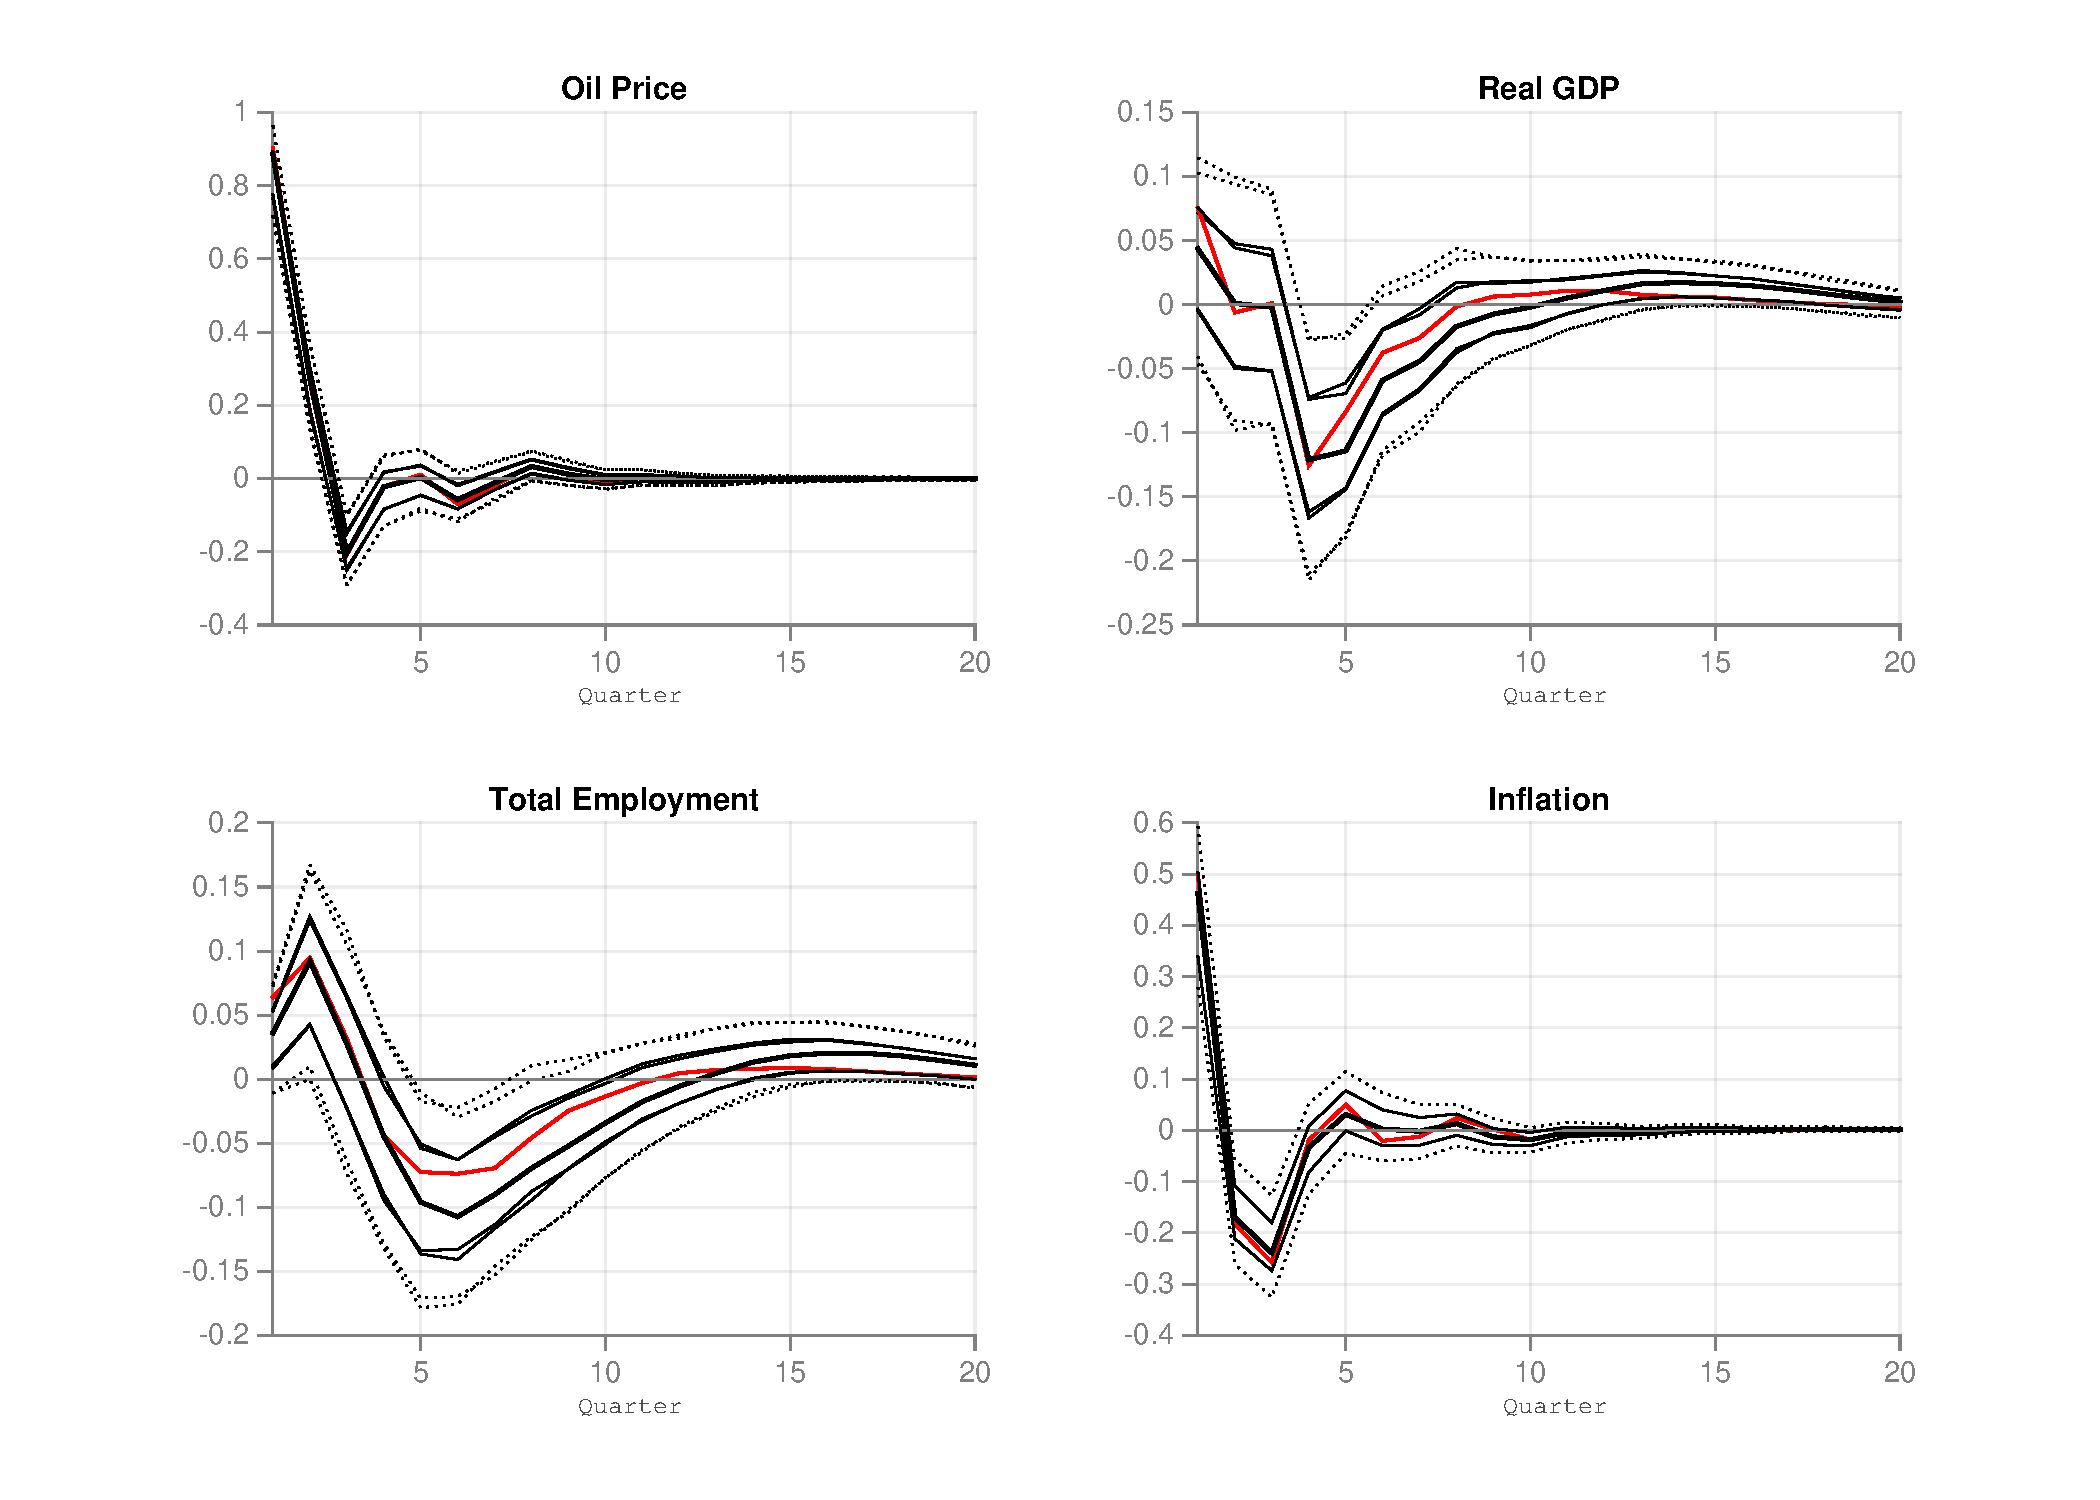
\includegraphics[width=7.5cm]{Figures/Robustness_3lags} &  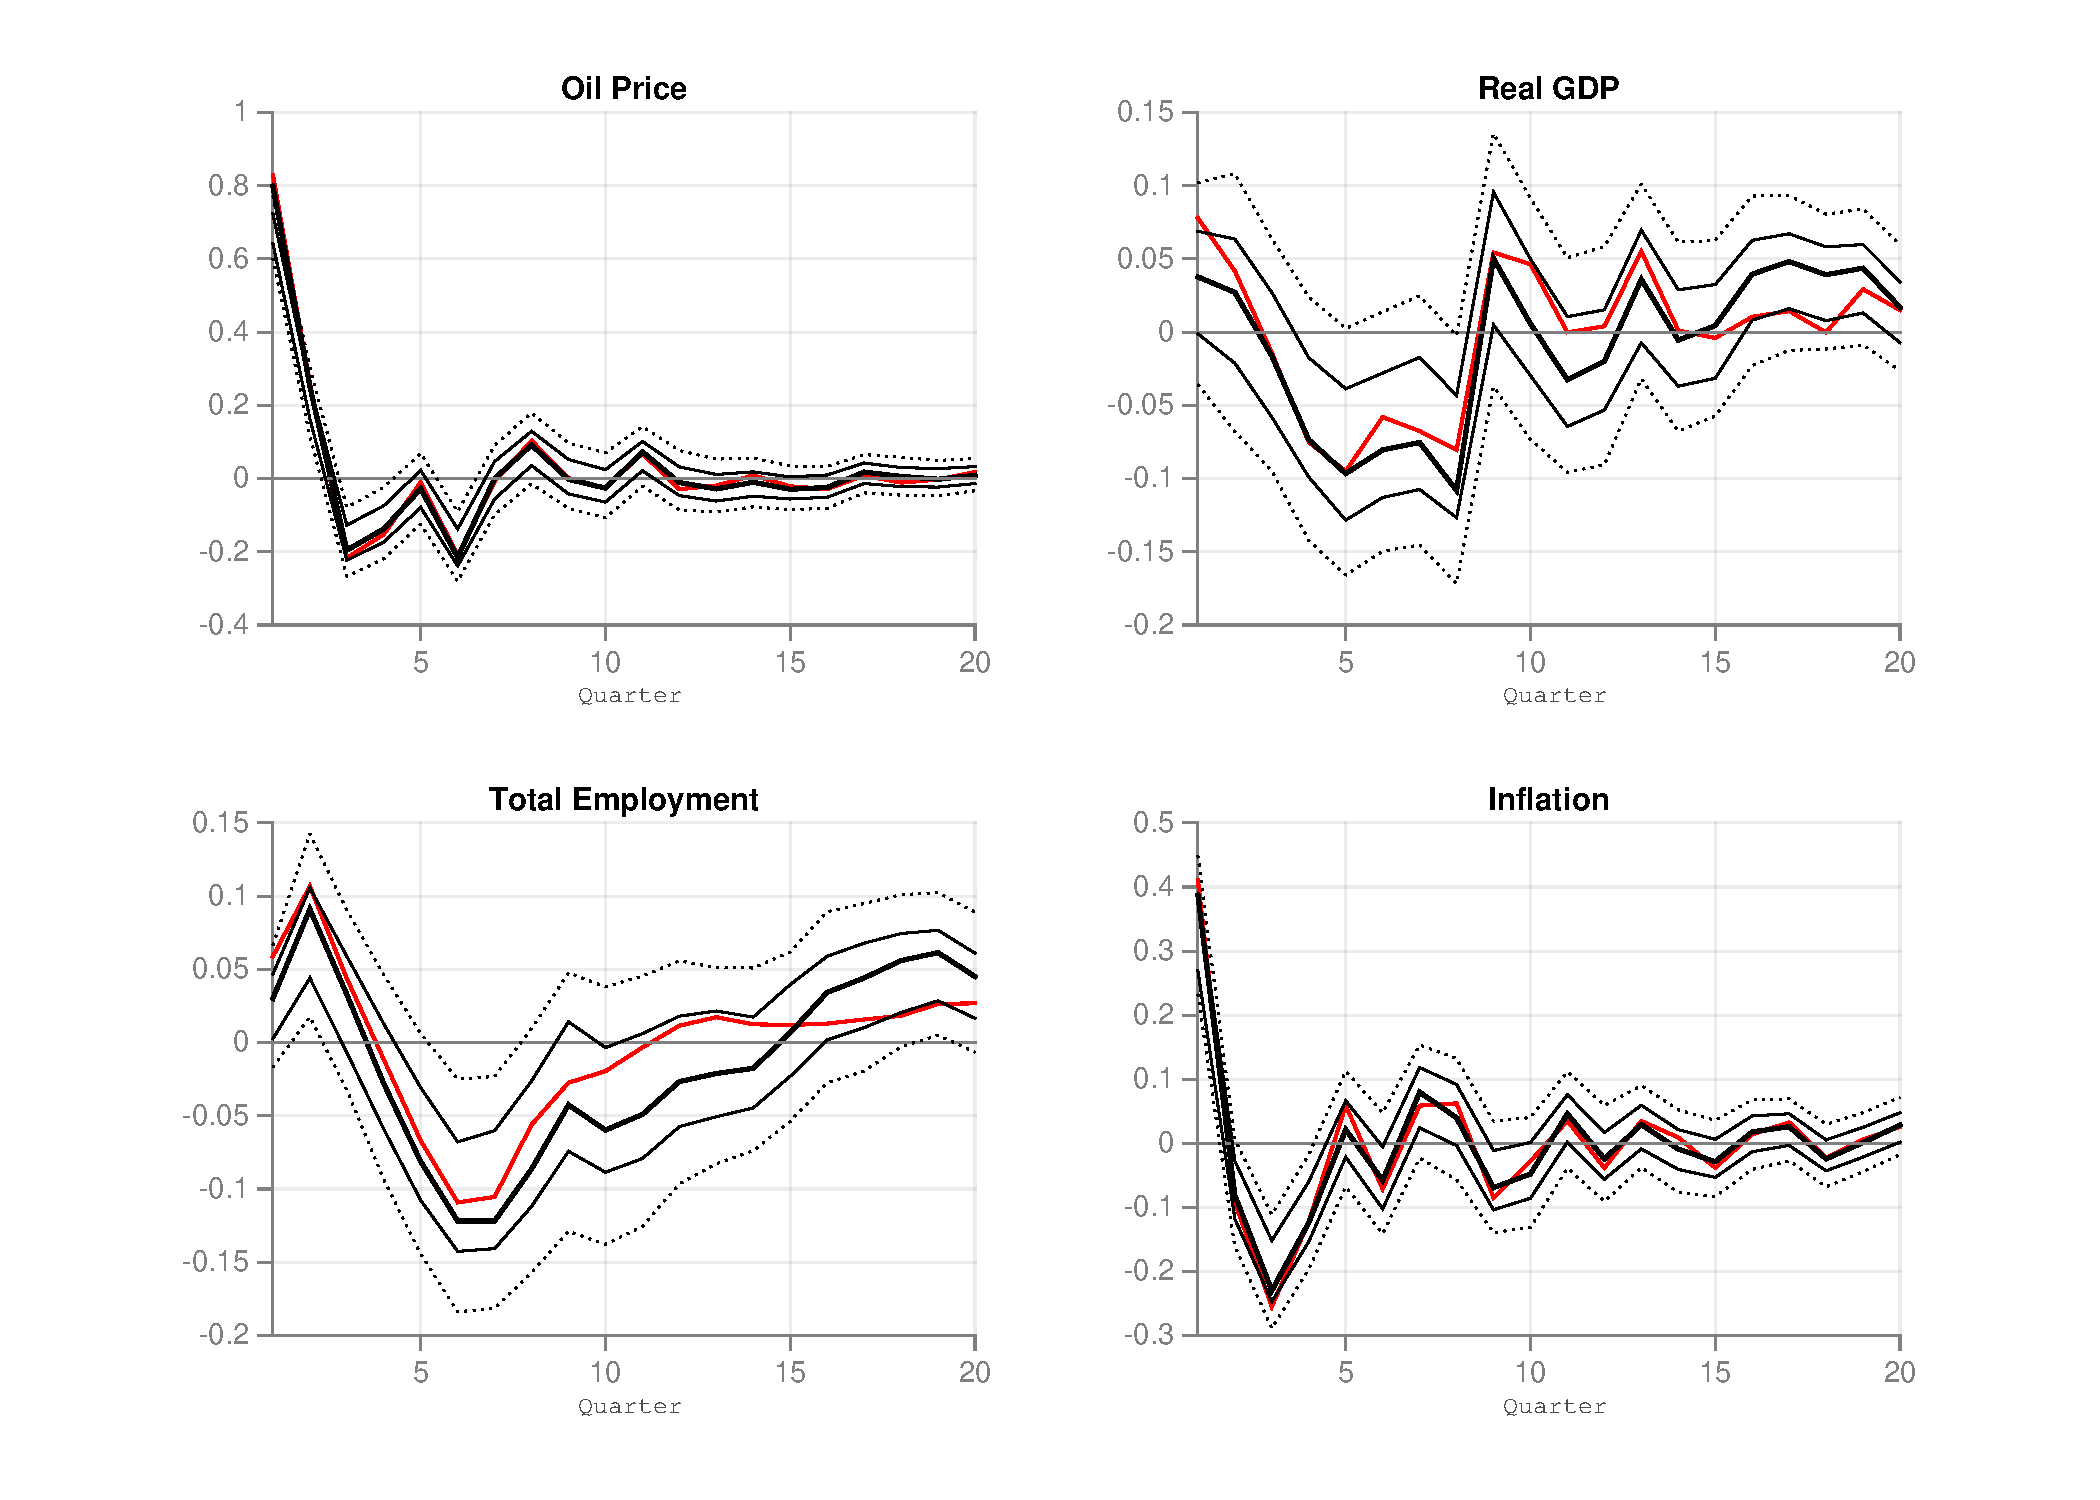
\includegraphics[width=7.5cm]{Figures/Robustness_8lags}&
				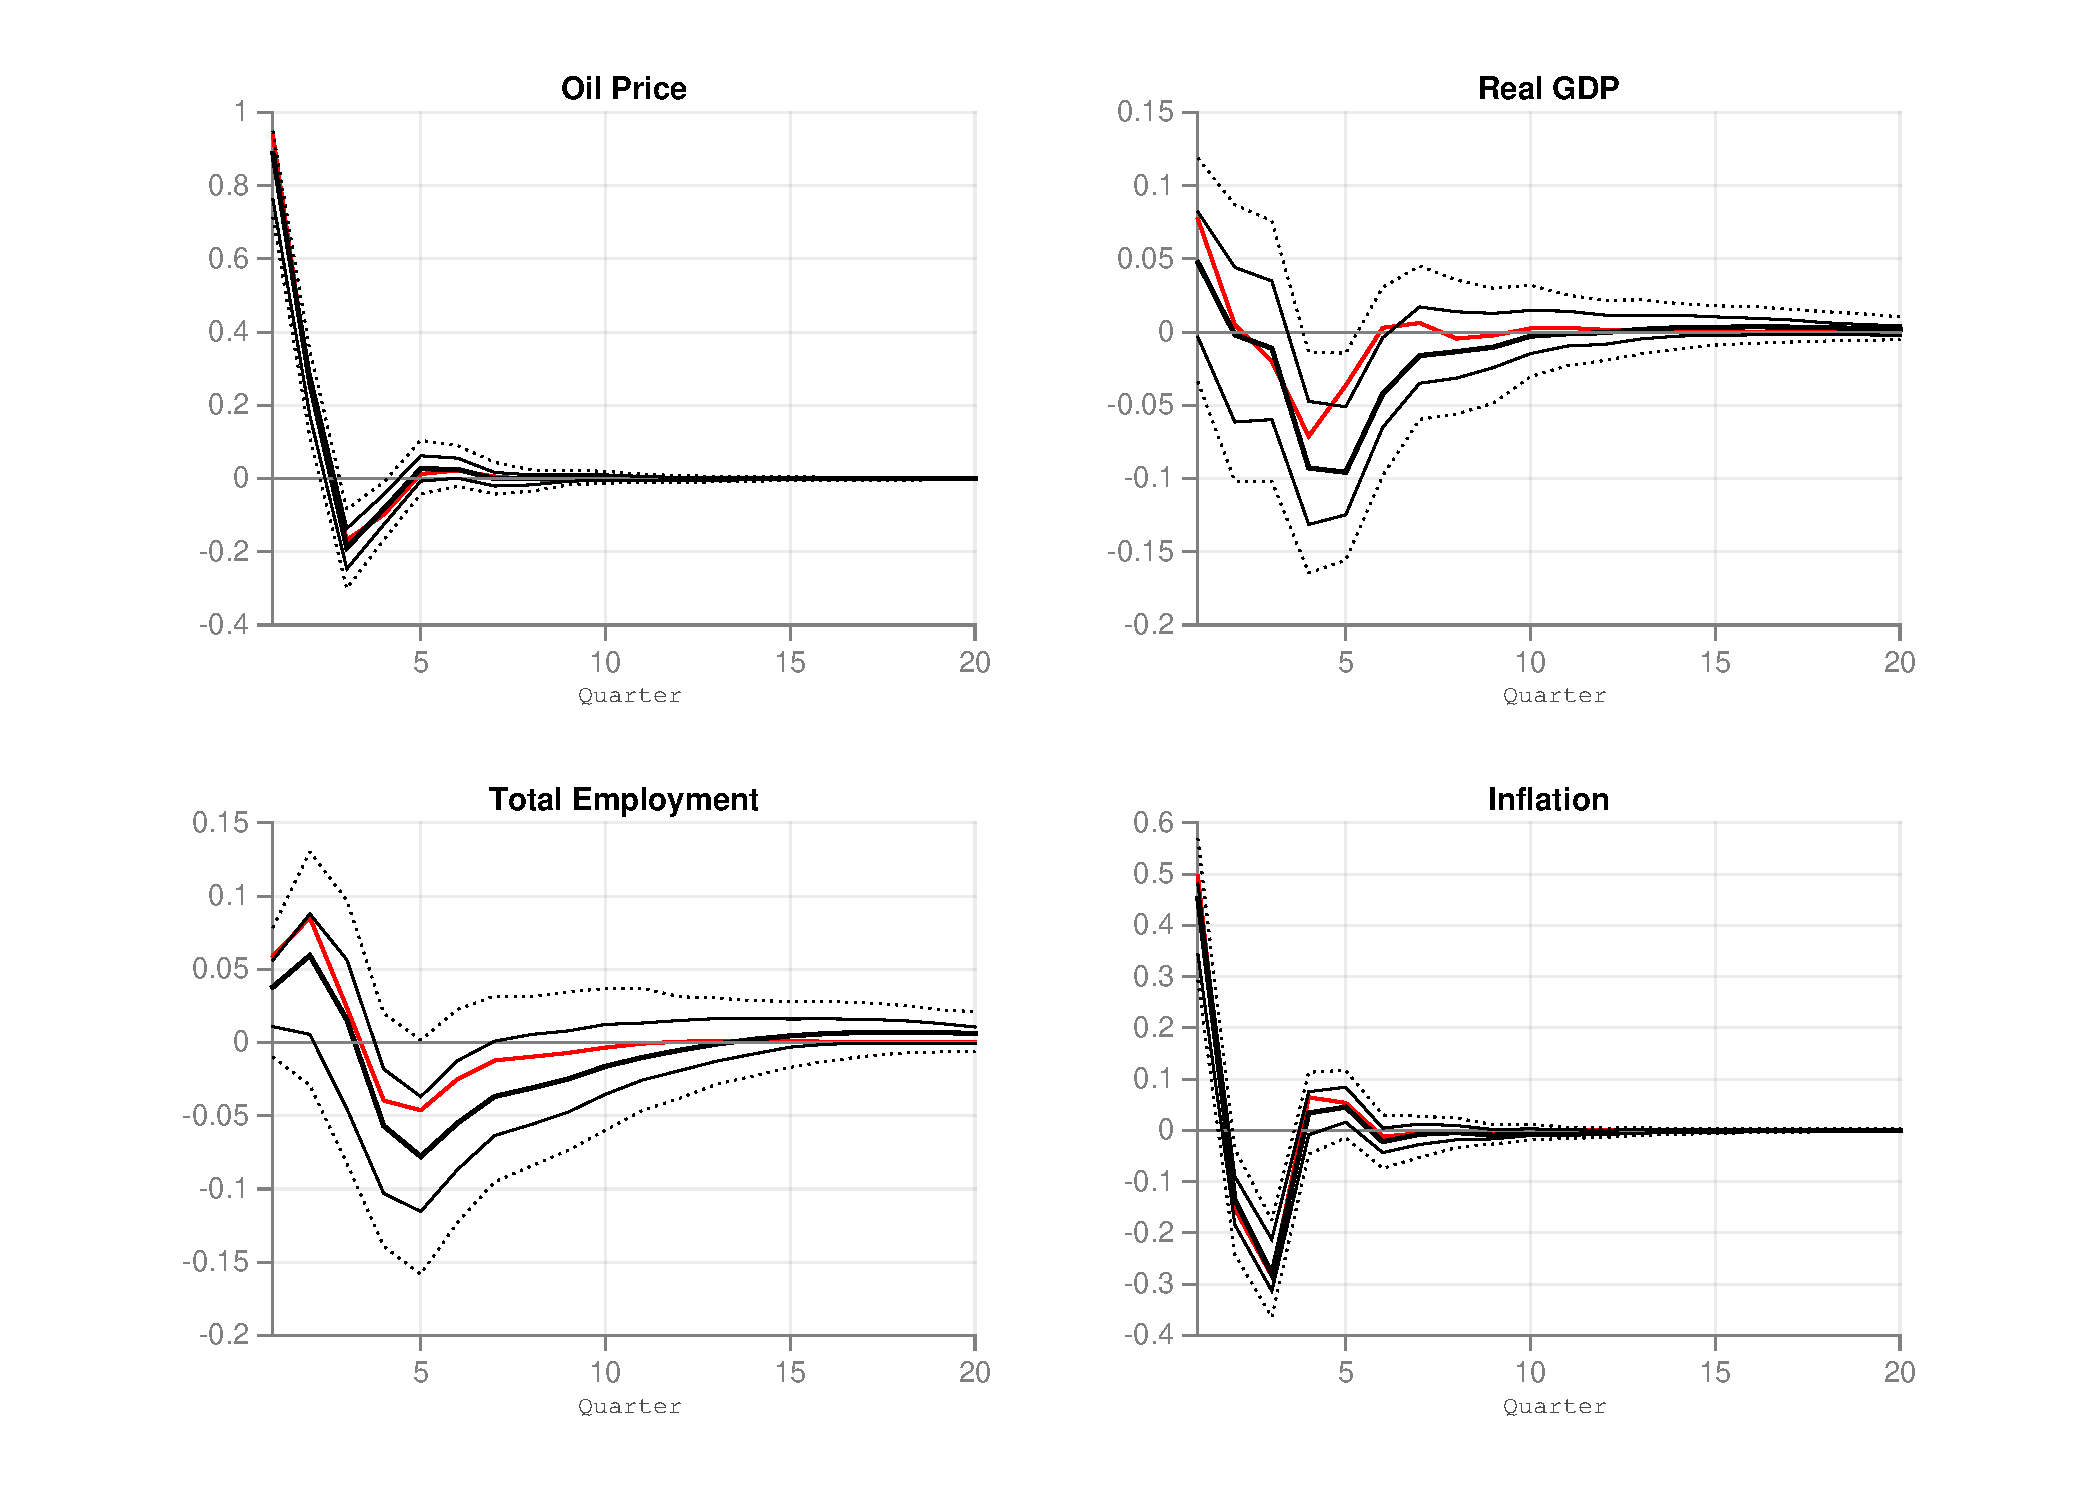
\includegraphics[width=7.5cm]{Figures/Robustness_3factors} 			
			\end{tabular}
		\end{center}
		\footnotesize{\emph{Notes:  
				This figure presents structural impulse response functions from the FAVAR (black solid line with 60\% and 90\% standard error bands) and the SVAR (red solid line) with respect to an oil price shock. 
				The variables included in the SVAR are:  growth rate of  oil price,  growth rate of real GDP,  growth rate of total employment,  change in inflation and  change in interest rate.
				We construct the FAVAR by augmenting the initial SVAR with two factors computed using principal component analysis from a data set of 106 variables describing the US economy. We identify this structural shock by ranking oil price first the FAVAR.
				Panel A considers only the period before the great moderation, from 1959:Q1 to 1984:Q3. 
				Panel B considers only the period after the great moderation, from 1985:Q1 to 2014:Q3. 
				Panel C omits the Zelo-Lower-Bound period, from 1959:Q1 to 2008:Q3.
				Panel D considers both models with a number of 3 lags instead of two.
				Panel E considers both models with a number of 8 lags.
				Panel F considers the FAVAR with a number of 3 factors included instead of two.
			}}	
		\end{figure}
	\end{landscape}
	
	
	

\newpage

\begin{landscape}
	\begin{figure}[H]
		\begin{center}
			\caption{\textsc{Robustness checks: Lag comparison}}
			\label{fig:robustness_lags}
			\begin{tabular}{ccc}
			\multirow{ 4}{6cm}{
			\emph{Notes:  
				This figure presents a comparison between the impulse response functions of SVAR and FAVAR with 2 or 3 lags.
				It can be observed that with 3 lags FAVAR and SVAR are more similar but they suffer from more noise		}
			} &
				A. SVAR 2 lags & B. SVAR 3 lags  \\
				&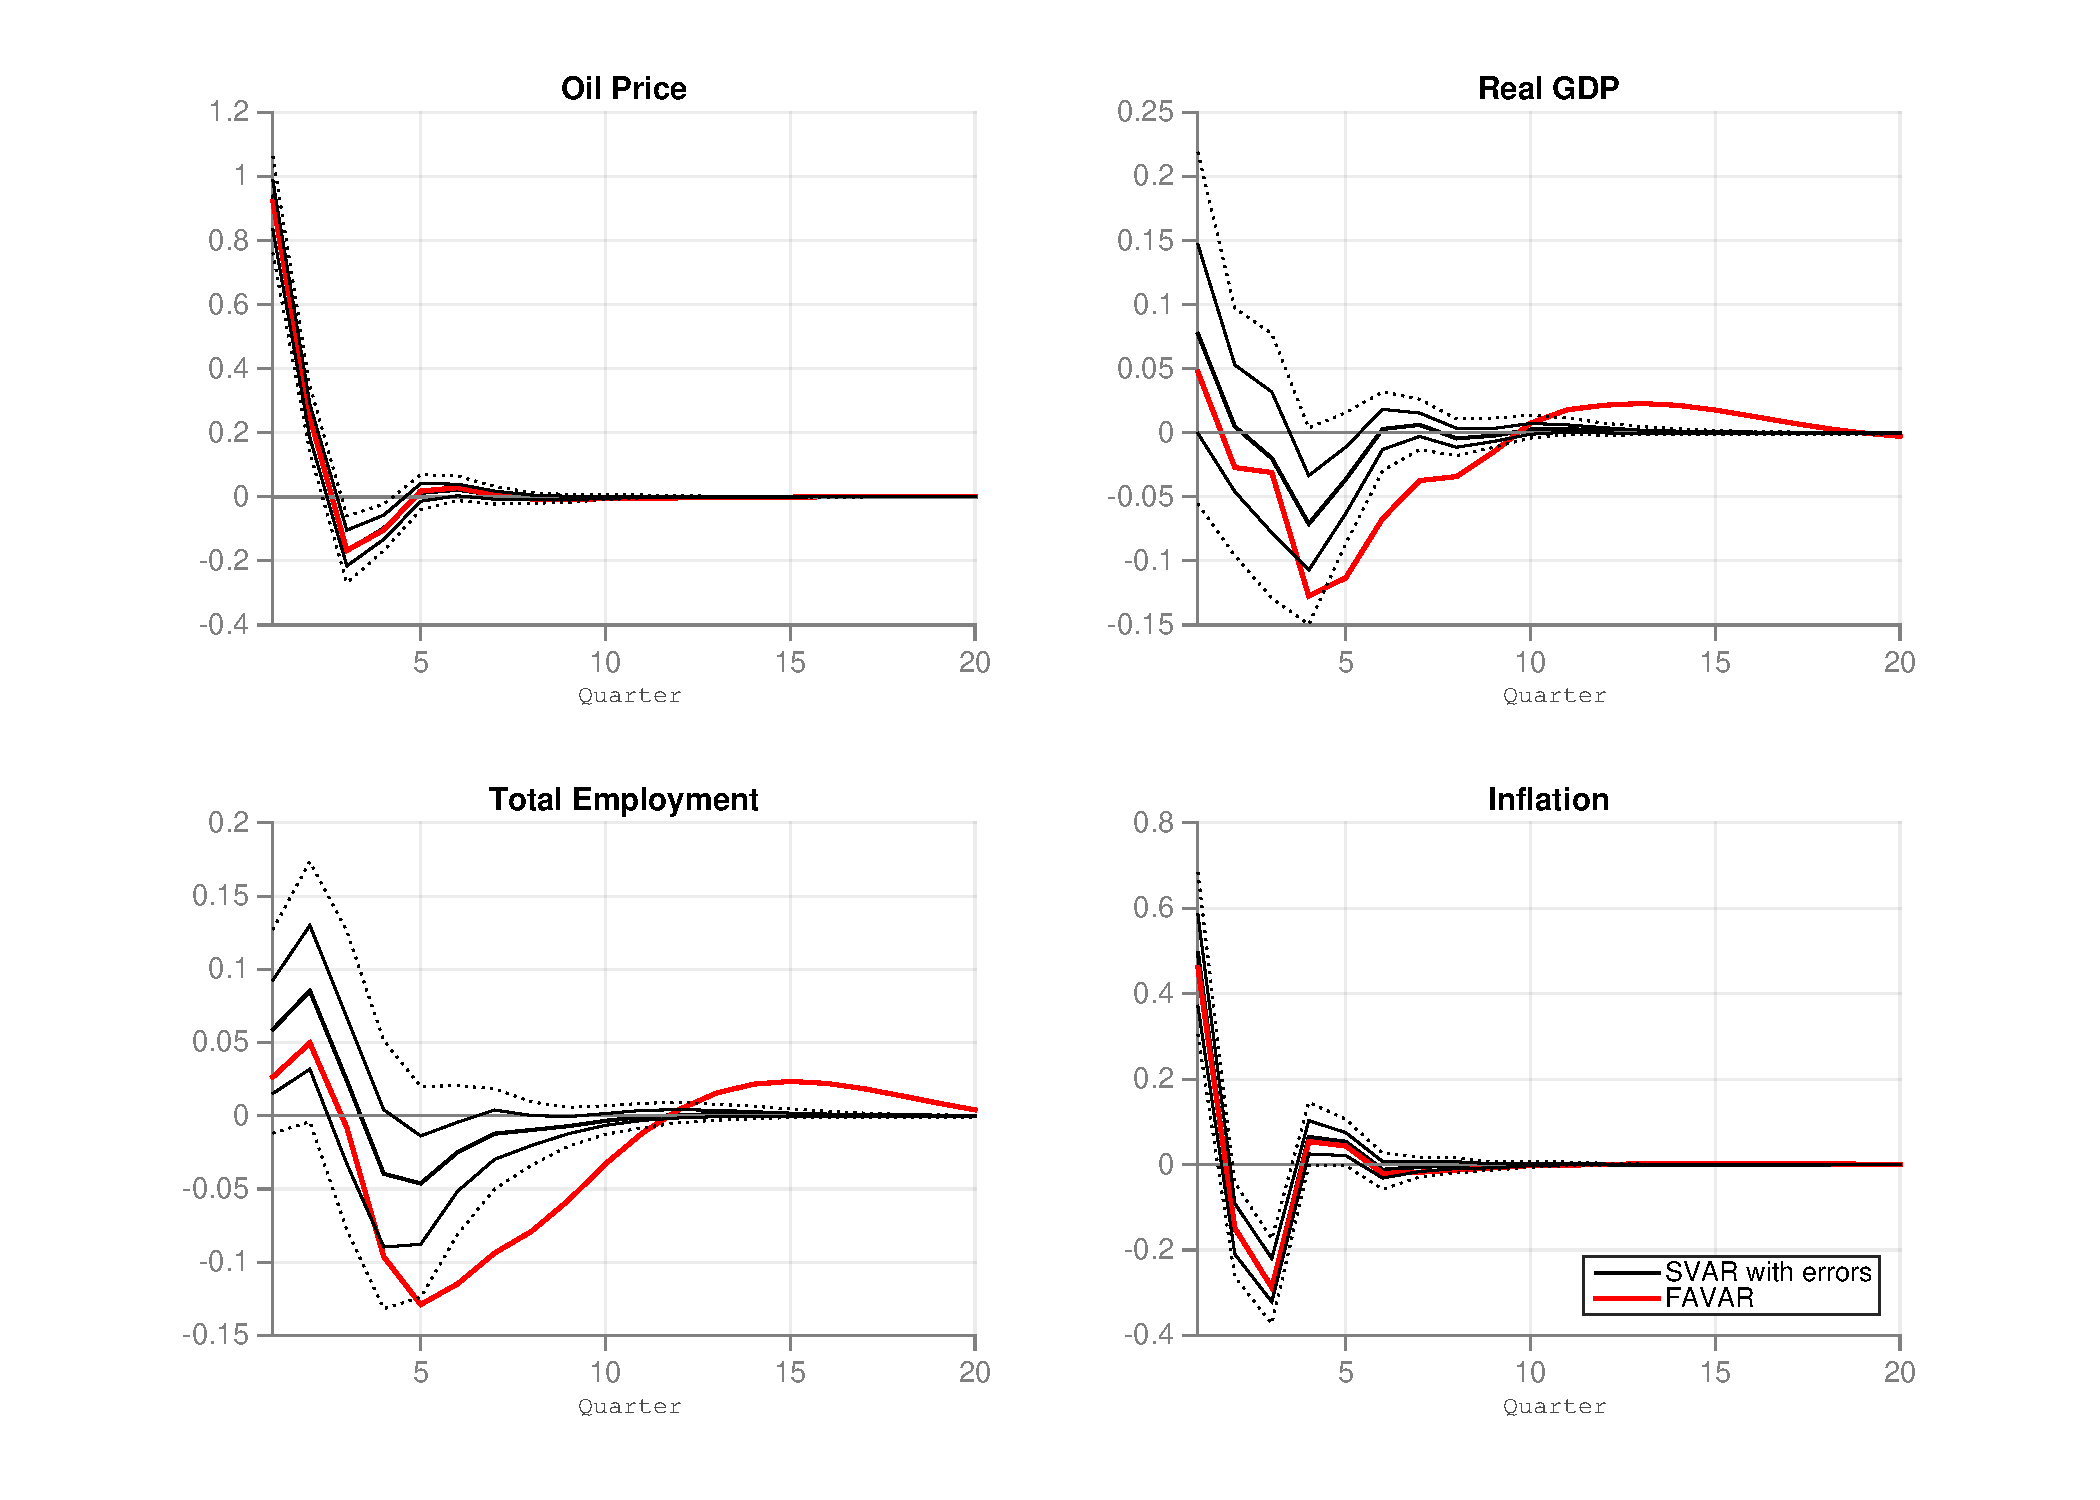
\includegraphics[width=9cm]{Figures/rob_SVAR_2} &  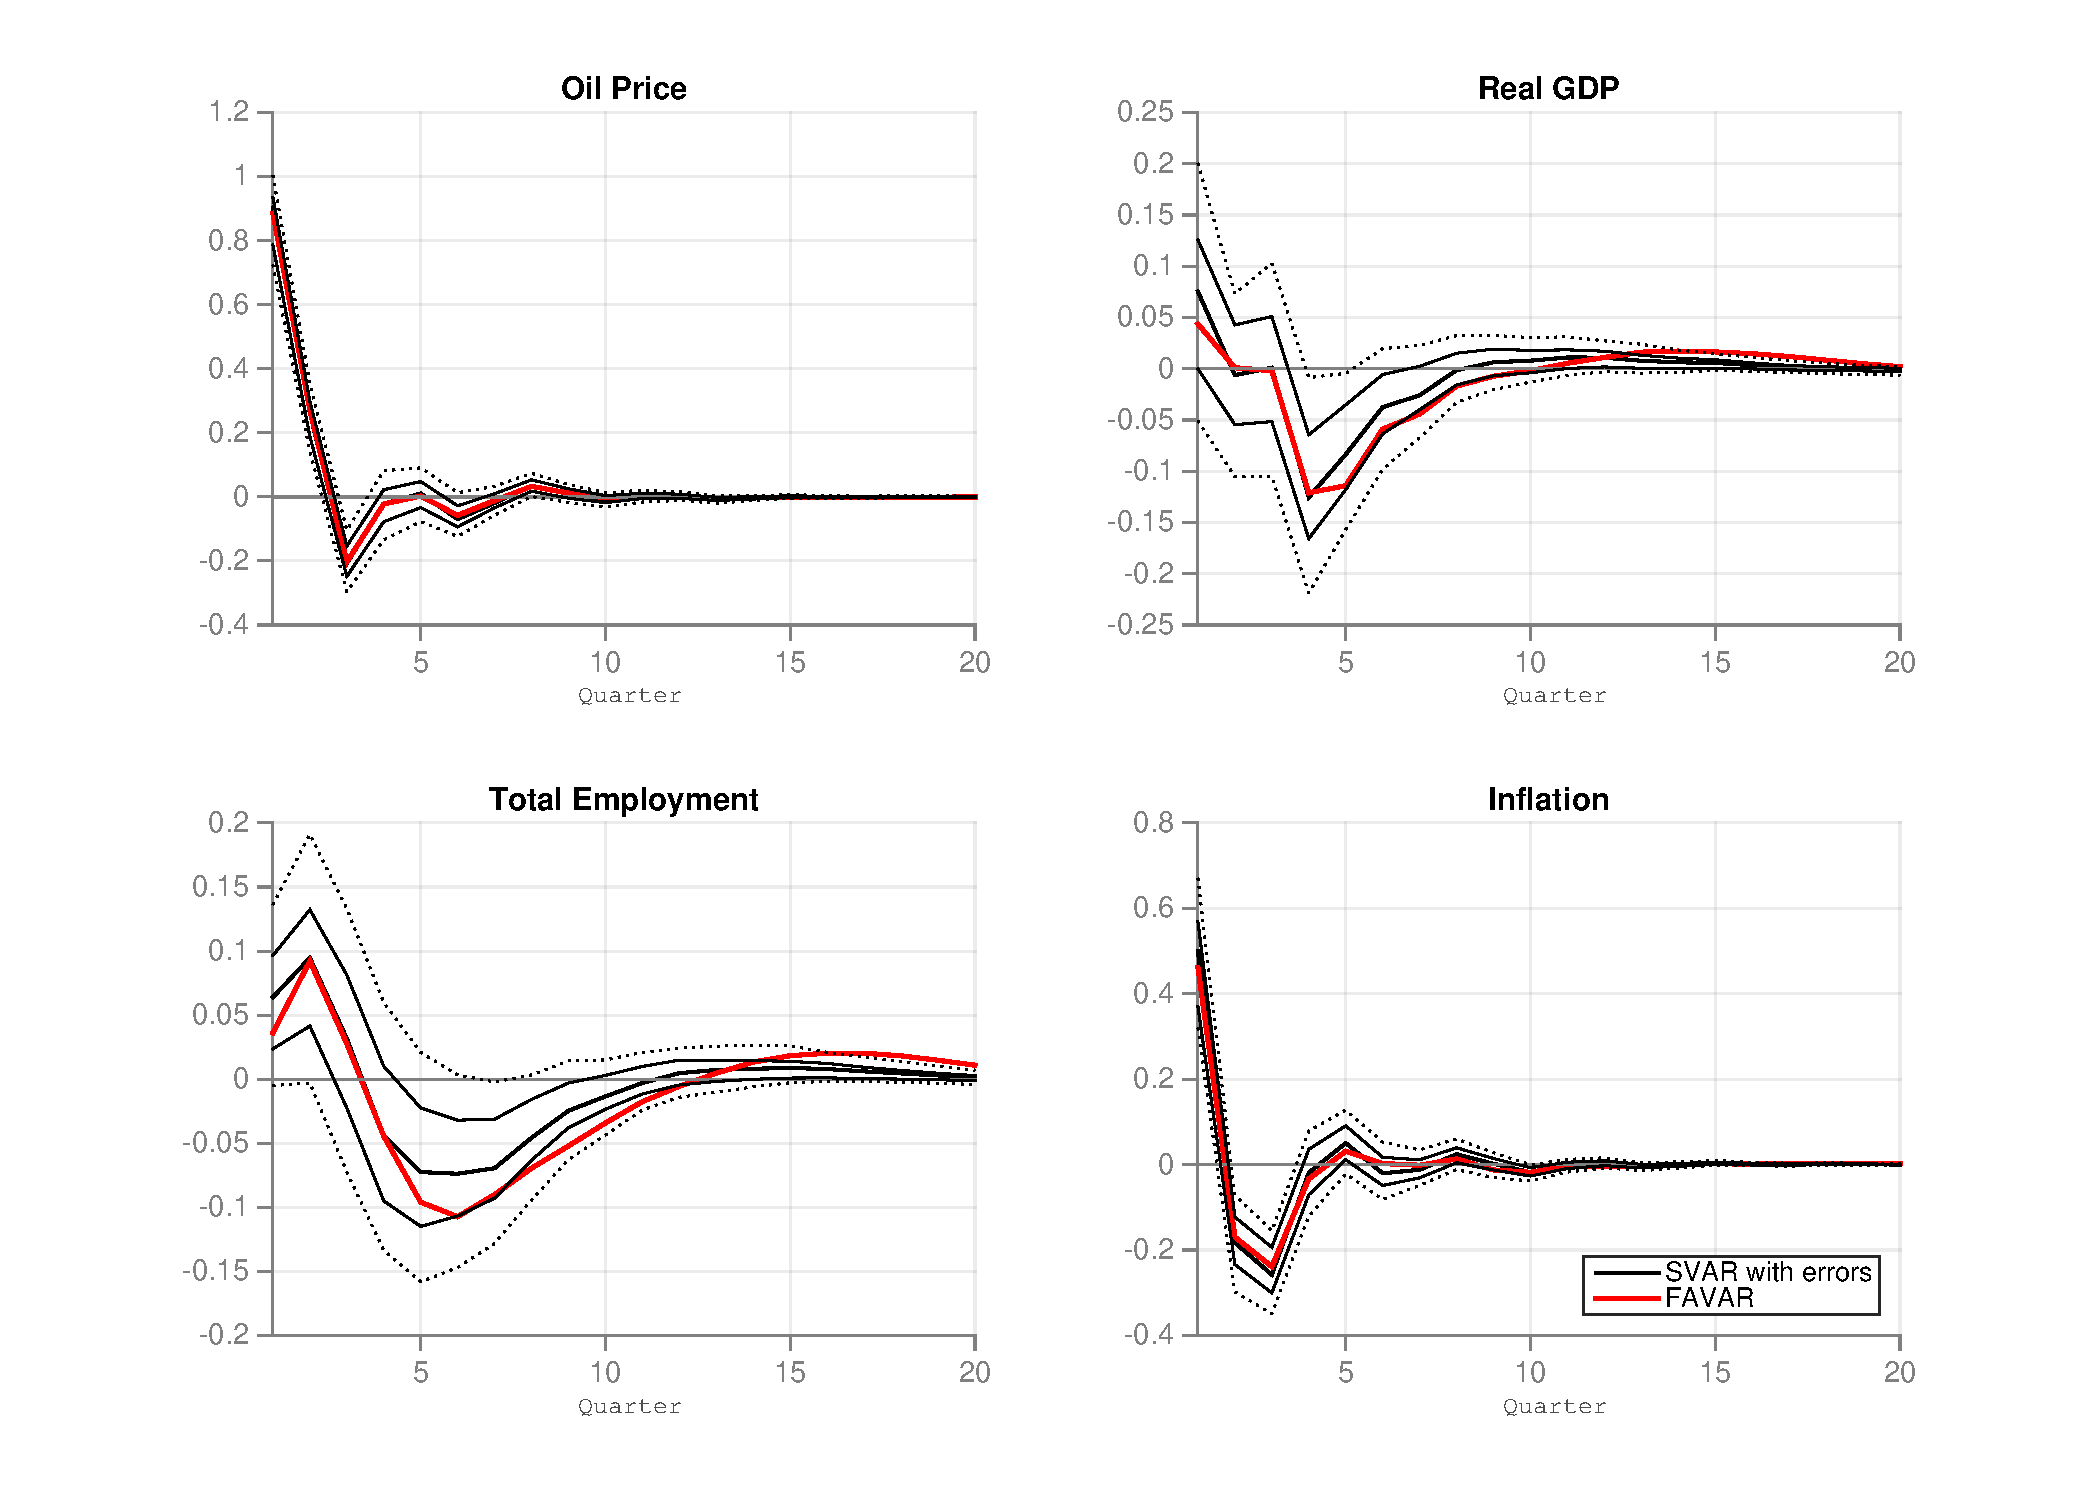
\includegraphics[width=9cm]{Figures/rob_SVAR_3} \\
				&D. FAVAR 2 lags  & E. FAVAR 3 lags  \\
				&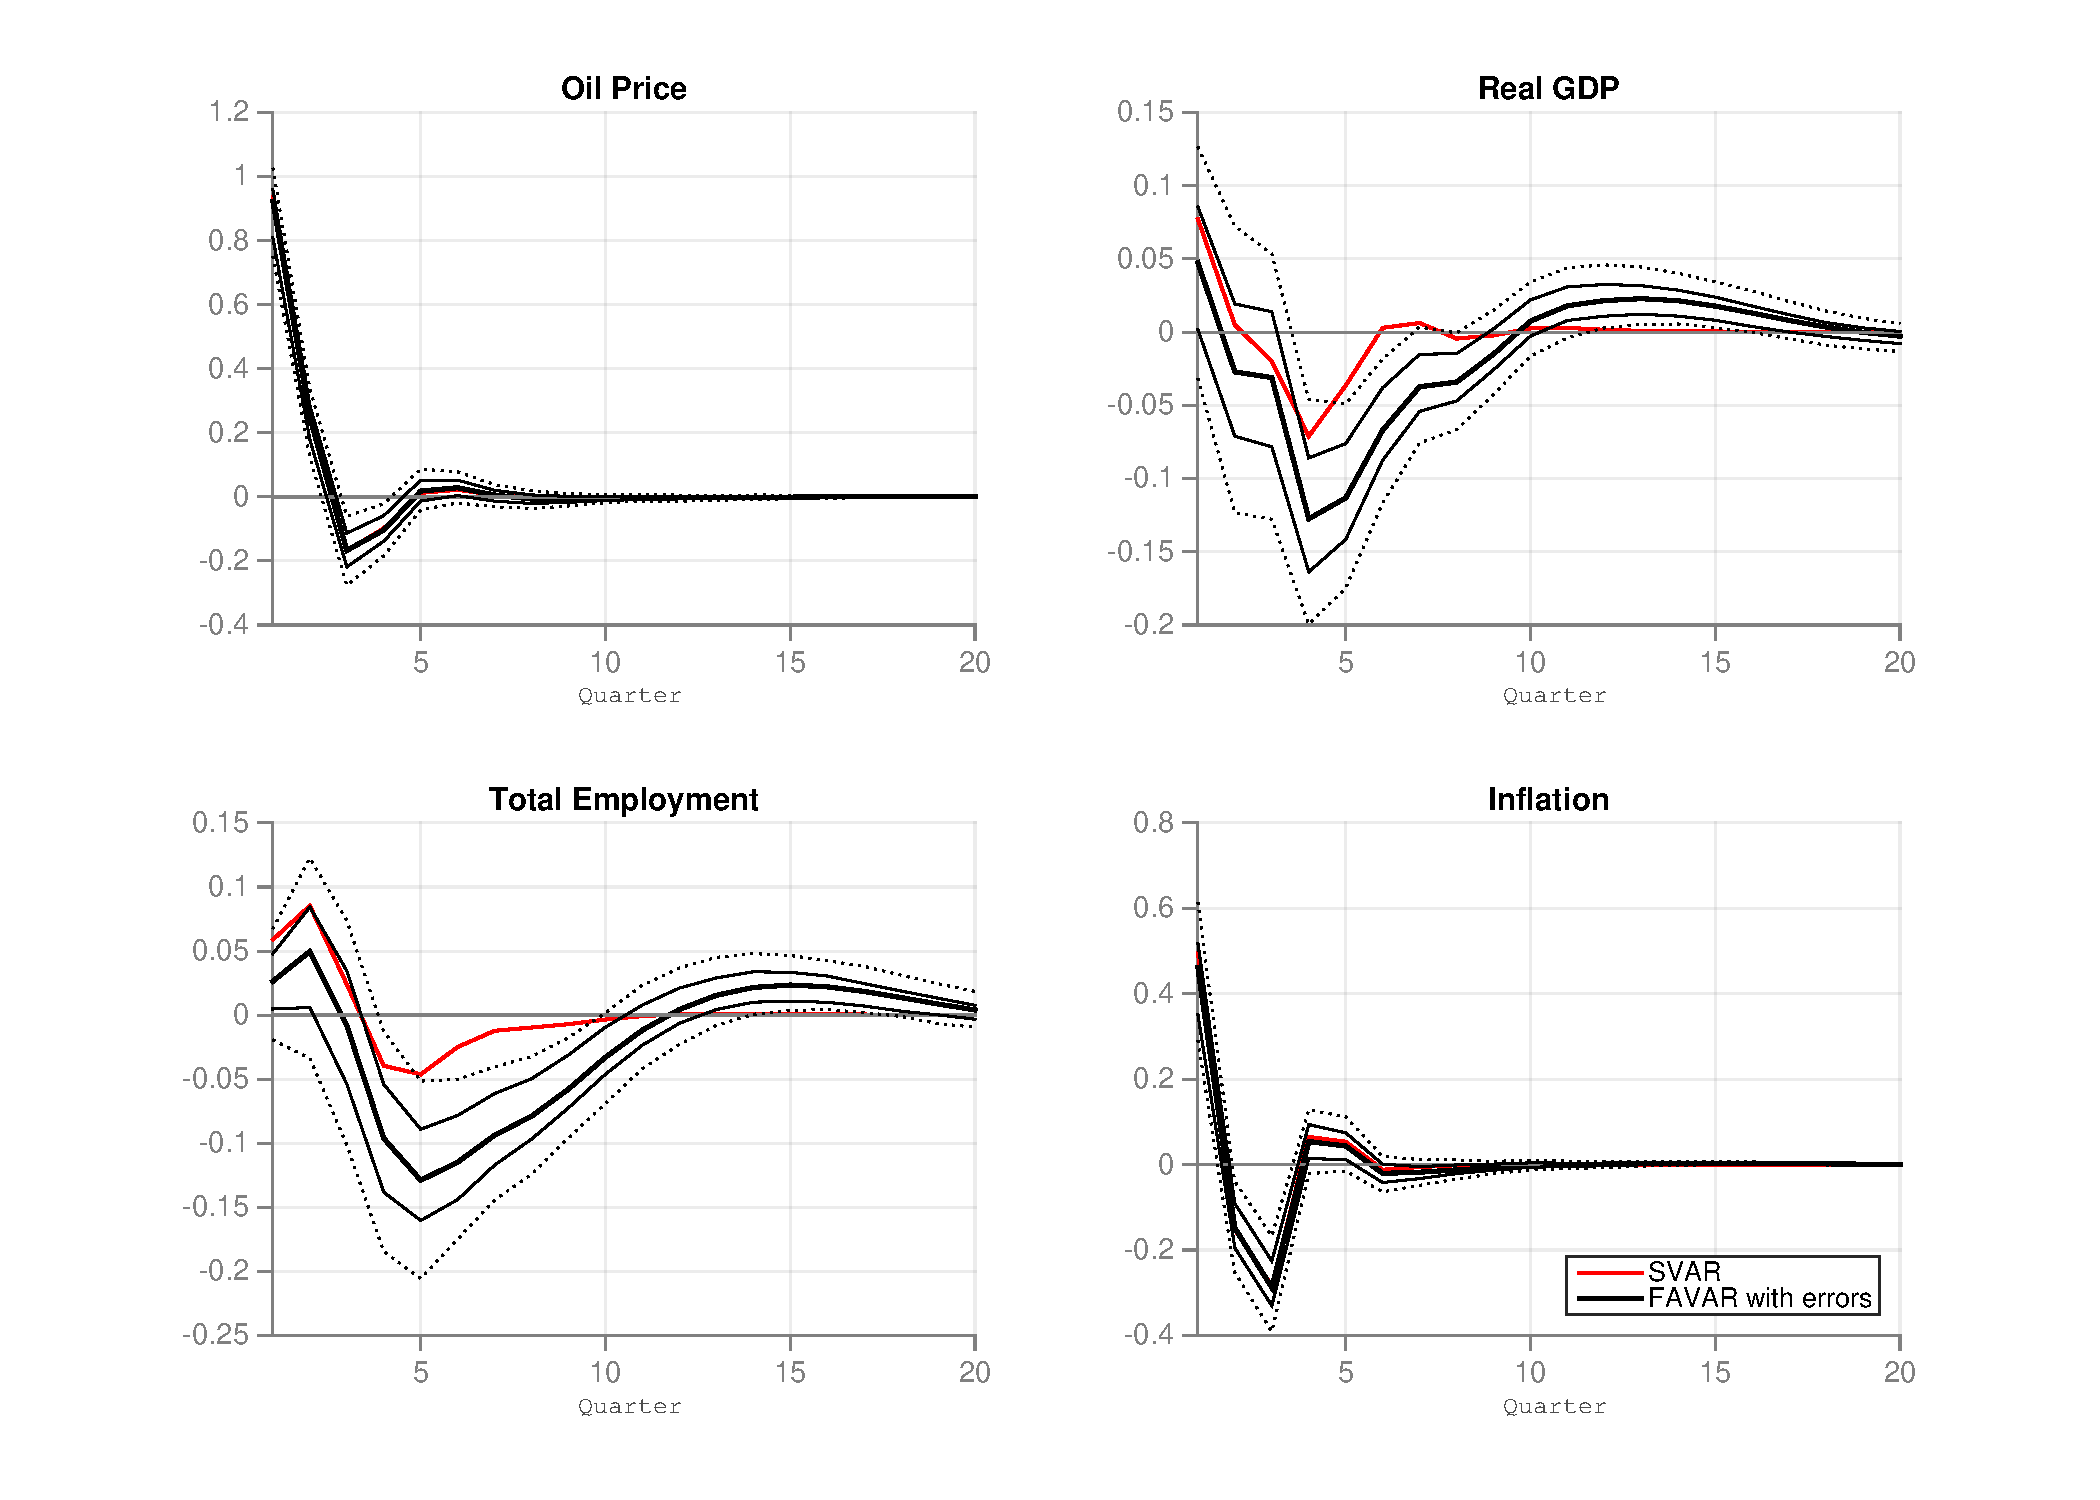
\includegraphics[width=9cm]{Figures/rob_FAVAR_2} &  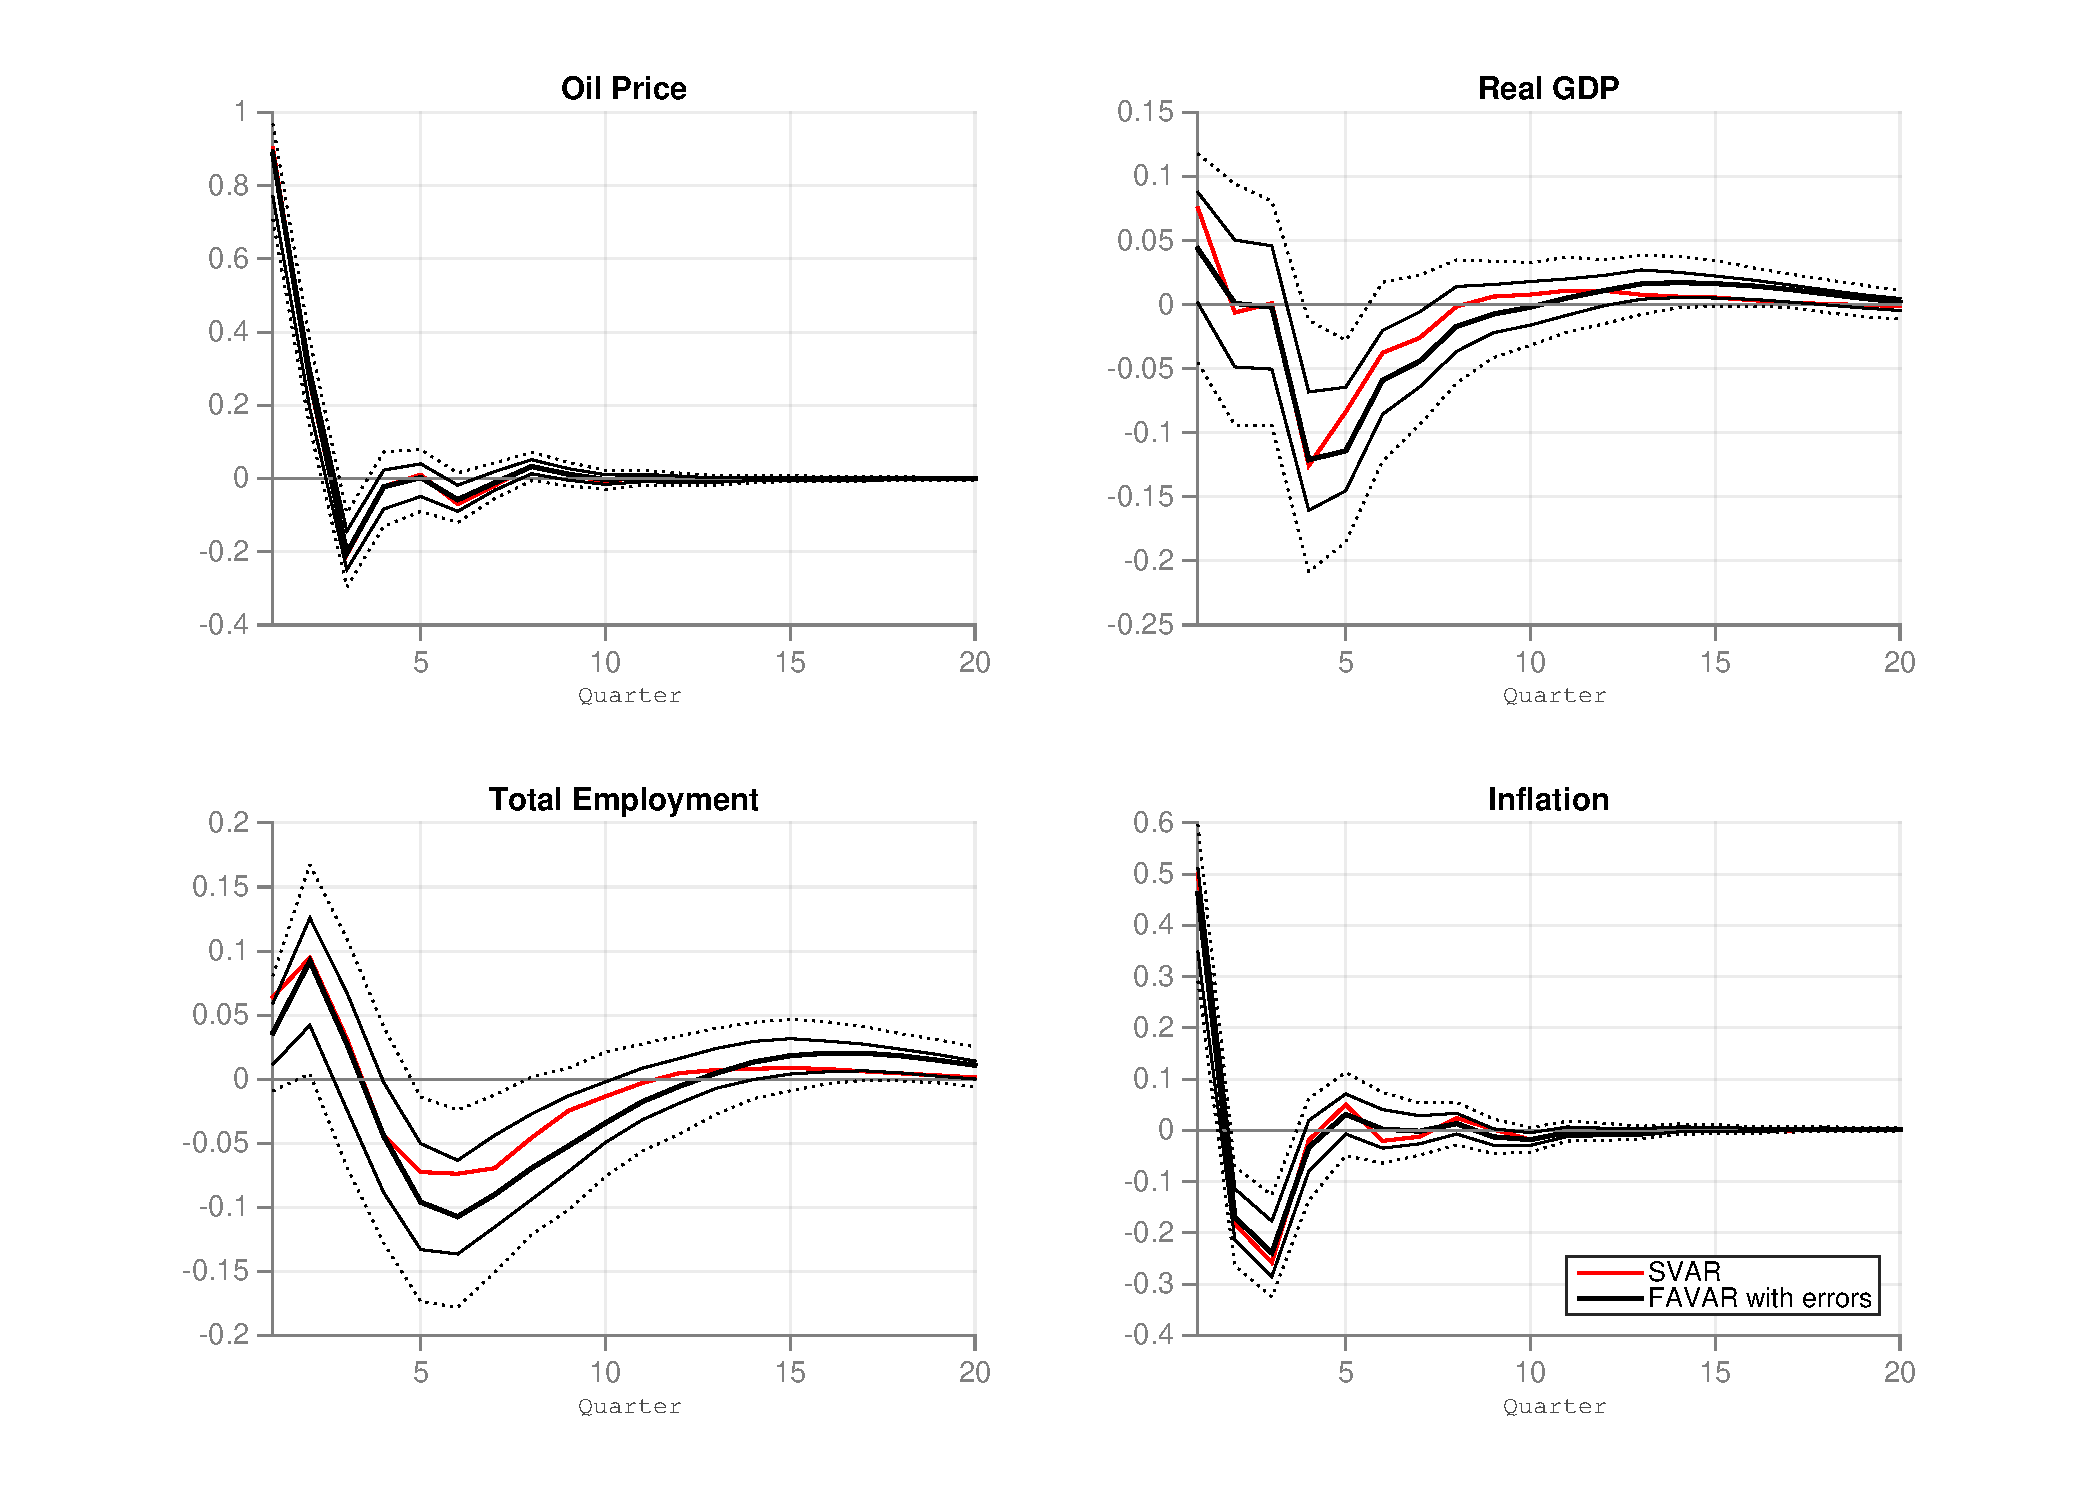
\includegraphics[width=9cm]{Figures/rob_FAVAR_3}			\end{tabular}
		\end{center}
		\end{figure}
	\end{landscape}


	%\begin{figure}[H]
	%	\begin{center}
	%		\caption{\textsc{Without ZLB period}}
	%		%		\label{fig:FAVAR_irf}
	%		\includegraphics[width=15cm]{Figures/FAVAR_robust_1}
	%	\end{center}
	%	\footnotesize{Notes:
	%		This figure presents structural impulse response functions from the FAVAR (black solid line with 60\% and 90\% standard error bands) and SVAR (red solid line) with respect to an oil price shock. We identify this structural shock by ranking oil price first the the FAVAR.
	%	}
	%\end{figure}
	%
	%\begin{figure}[H]
	%	\begin{center}
	%		\caption{\textsc{Before Great Moderation}}
	%		%		\label{fig:FAVAR_irf}
	%		\includegraphics[width=15cm]{Figures/FAVAR_robust_2a}
	%	\end{center}
	%	\footnotesize{Notes:
	%		This figure presents structural impulse response functions from the FAVAR (black solid line with 60\% and 90\% standard error bands) and SVAR (red solid line) with respect to an oil price shock. We identify this structural shock by ranking oil price first the the FAVAR.
	%	}
	%\end{figure}
	%
	%\begin{figure}[H]
	%	\begin{center}
	%		\caption{\textsc{After Great Moderation}}
	%		%		\label{fig:FAVAR_irf}
	%		\includegraphics[width=15cm]{Figures/FAVAR_robust_2b}
	%	\end{center}
	%	\footnotesize{Notes:
	%		This figure presents structural impulse response functions from the FAVAR (black solid line with 60\% and 90\% standard error bands) and SVAR (red solid line) with respect to an oil price shock. We identify this structural shock by ranking oil price first the the FAVAR.
	%	}
	%\end{figure}
	
	
	%\begin{figure}[H]
	%	\begin{center}
	%		\caption{\textsc{2 Lags}}
	%		%		\label{fig:FAVAR_irf}
	%		\includegraphics[width=0.5\textheight]{Figures/FAVAR_robustLag2}
	%	\end{center}
	%	\footnotesize{Notes:
	%		This figure presents structural impulse response functions from the FAVAR (black solid line with 60\% and 90\% standard error bands) and SVAR (red solid line) with respect to an oil price shock. We identify this structural shock by ranking oil price first the the FAVAR.
	%	}
	%\end{figure}
	%
	%\begin{figure}[H]
	%	\begin{center}
	%		\caption{\textsc{4 Lags}}
	%		%		\label{fig:FAVAR_irf}
	%		\includegraphics[width=0.5\textheight]{Figures/FAVAR_robustLag4}
	%	\end{center}
	%	\footnotesize{Notes:
	%		This figure presents structural impulse response functions from the FAVAR (black solid line with 60\% and 90\% standard error bands) and SVAR (red solid line) with respect to an oil price shock. We identify this structural shock by ranking oil price first the the FAVAR.
	%	}
	%\end{figure}
	
	
	%\begin{figure}[H]
	%	\begin{center}
	%		\caption{\textsc{5 Lags}}
	%		%		\label{fig:FAVAR_irf}
	%		\includegraphics[width=0.5\textheight]{Figures/FAVAR_robustLag5}
	%	\end{center}
	%	\footnotesize{Notes:
	%		This figure presents structural impulse response functions from the FAVAR (black solid line with 60\% and 90\% standard error bands) and SVAR (red solid line) with respect to an oil price shock. We identify this structural shock by ranking oil price first the the FAVAR.
	%	}
	%\end{figure}
	
	%\begin{minipage}[b]{\textwidth}
	%\begin{figure}[H]
	%	\begin{center}
	%		\caption{\textsc{1 Factor}}
	%		%		\label{fig:FAVAR_irf}
	%		\includegraphics[width=0.5\textheight]{Figures/FAVAR_robustFactor1}
	%	\end{center}
	%	\footnotesize{Notes:
	%		This figure presents structural impulse response functions from the FAVAR (black solid line with 60\% and 90\% standard error bands) and SVAR (red solid line) with respect to an oil price shock. We identify this structural shock by ranking oil price first the the FAVAR.
	%	}
	%\end{figure}
	%
	%\begin{figure}[H]
	%	\begin{center}
	%		\caption{\textsc{3 Factor}}
	%		%		\label{fig:FAVAR_irf}
	%		\includegraphics[width=0.5\textheight]{Figures/FAVAR_robustFactor3}
	%	\end{center}
	%	\footnotesize{Notes:
	%		This figure presents structural impulse response functions from the FAVAR (black solid line with 60\% and 90\% standard error bands) and SVAR (red solid line) with respect to an oil price shock. We identify this structural shock by ranking oil price first the the FAVAR.
	%	}
	%\end{figure}
	
	%\end{minipage}
	
	%\begin{minipage}[l]{\textwidth}
	%\begin{figure}[H]
	%	\begin{center}
	%		\caption{\textsc{4 Factor}}
	%		%		\label{fig:FAVAR_irf}
	%		\includegraphics[width=0.5\textheight]{Figures/FAVAR_robustFactor4}
	%	\end{center}
	%	\footnotesize{Notes:
	%		This figure presents structural impulse response functions from the FAVAR (black solid line with 60\% and 90\% standard error bands) and SVAR (red solid line) with respect to an oil price shock. We identify this structural shock by ranking oil price first the the FAVAR.
	%	}
	%\end{figure}
	%
	%\begin{figure}[H]
	%	\begin{center}
	%		\caption{\textsc{5 Factor}}
	%		%		\label{fig:FAVAR_irf}
	%		\includegraphics[width=0.5\textheight]{Figures/FAVAR_robustFactor5}
	%	\end{center}
	%	\footnotesize{Notes:
	%		This figure presents structural impulse response functions from the FAVAR (black solid line with 60\% and 90\% standard error bands) and SVAR (red solid line) with respect to an oil price shock. We identify this structural shock by ranking oil price first the the FAVAR.
	%	}
	%\end{figure}
	%\end{minipage}
	
	\restoregeometry
	
\end{document}